\documentclass[conference]{IEEEtran}
\IEEEoverridecommandlockouts
% The preceding line is only needed to identify funding in the first footnote. If that is unneeded, please comment it out.
\usepackage{cite}
\usepackage{amsmath,amssymb,amsfonts}
\usepackage{algorithmic}
\usepackage{booktabs}
\usepackage{graphicx}
\usepackage{subcaption} % Import the package
\usepackage{textcomp}
\usepackage{xcolor}
\usepackage{multirow}
\usepackage{svg}
\usepackage{subfigure}
\usepackage{parskip}
\usepackage{booktabs}
\usepackage{threeparttable} % 添加这一行来导入 threeparttable 宏包
\def\BibTeX{{\rm B\kern-.05em{\sc i\kern-.025em b}\kern-.08em
    T\kern-.1667em\lower.7ex\hbox{E}\kern-.125emX}}
\begin{document}
\title{INT104 Lab Report}
\author{Zhibin Jiang Student-ID: 2360003 E-Mail: zhibin.jiang23@student.xjtlu.edu.cn}
\maketitle
%**摘要**：本文档是一份LaTeX模板及使用说明。
%本文档与IEEEtran.cls文件共同定义了论文的各个组成部分（标题、正文、标题栏等）。
%**重要提示：论文标题和摘要中请勿使用符号、特殊字符、脚注或数学公式**。摘要字数应控制在100到150字左右，且必须与电子提交的摘要文本完全一致。 
%\begin{abstract}
%This is an abstract.
%\end{abstract}
% 关键词
\begin{IEEEkeywords}
Spearman Correlation Matrix,
Shapiro-Wilk Test,
Robust Standardization,
Logarithmic Transformation,
Box-Cox Transformation,
Principal Component Analysis,
K-Means,
DBSCAN,
Gaussian Mixture Model (GMM),
Confusion Matrix,
Logistic Regression,
Boosting-Based Classifiers,
Transformer Classifier
\end{IEEEkeywords}



\section{\textbf{Introduction}}
%本文将会按照数据观察及标准化(Task I)、无监督学习(Task II)和监督学习(Task III)的顺序进行。
%在数据观察部分首先会根据Spearman Correlation Matrix 评估一些不参与特征组合的特征例如\textit{Gender}，随后使用 Shapiro-Wiki Test 解释为什么不使用Z-Score标准化，最终选择出了 Robust Standarization, Logarithmic 以及 Box-Cox Standarization. 
%在无监督学习部分首先介绍了特征选择的原因以及特征组合，并且引入了两种评估聚类的方式分别是带标签的聚类评估 Adjusted Rand Index (ARI) 和不带标签的聚类评估 Davies Bouldin Index (DBI) 。基于这两种评估方法，我们测试了 K-Means, DBSCAN 以及 GMM聚类的效果。
%在监督学习部分通过组合更多中特征对三种不同类别的classifier进行准确率测试，分别是逻辑回归, Boosting-based 以及 Transformer classifier model. 并且通过混淆矩阵来分析每个模型的特点.最后的结论会解释一些在前文中的发现例如特征选择和标准化的差异。

This report proceeds in the order of Data Observation and Standardization (Task I), Unsupervised Learning (Task II), and Supervised Learning (Task III).  
In the data observation section, we first evaluate features not involved in feature combination (e.g., \textit{Gender}) using the Spearman Correlation Matrix. Subsequently, we explain why Z-Score standardization is not adopted via the Shapiro-Wilk Test, ultimately selecting Robust Standardization, Logarithmic Transformation, and Box-Cox Standardization.  
In the unsupervised learning section, we first introduce the rationale for feature selection and feature combination, followed by two clustering evaluation methods: the label-based Adjusted Rand Index (ARI) and the label-free Davies-Bouldin Index (DBI). Based on these metrics, we test the performance of K-Means, DBSCAN, and Gaussian Mixture Model (GMM) clustering algorithms.  
In the supervised learning section, we conduct accuracy tests on three categories of classifiers—Logistic Regression, Boosting-based models, and Transformer classifier models—by incorporating more combined features. We analyze the characteristics of each model using confusion matrices. The final conclusion interprets key findings from preceding sections, such as differences in feature selection and standardization approaches.

\section{\textbf{Task I \& II: Data Observation \& Data Standardize}}
%数据一共有466行,无空值和缺失值。数据包含8个特征，分别为
There are 466 rows in the data set with no null or missing values. The data set contains 8 features, which are \textit{Programme}, \textit{Gender},\textit{Grade}, \textit{Q1}, \textit{Q2}, \textit{Q3}, \textit{Q4}, \textit{Q5}.
% 使用 Spearman correlation 矩阵检查8个特征之间的相关性
Check the correlations among the eight features using a \textbf{Spearman Correlation Matrix}.
\begin{figure}[h!]
    \centerline{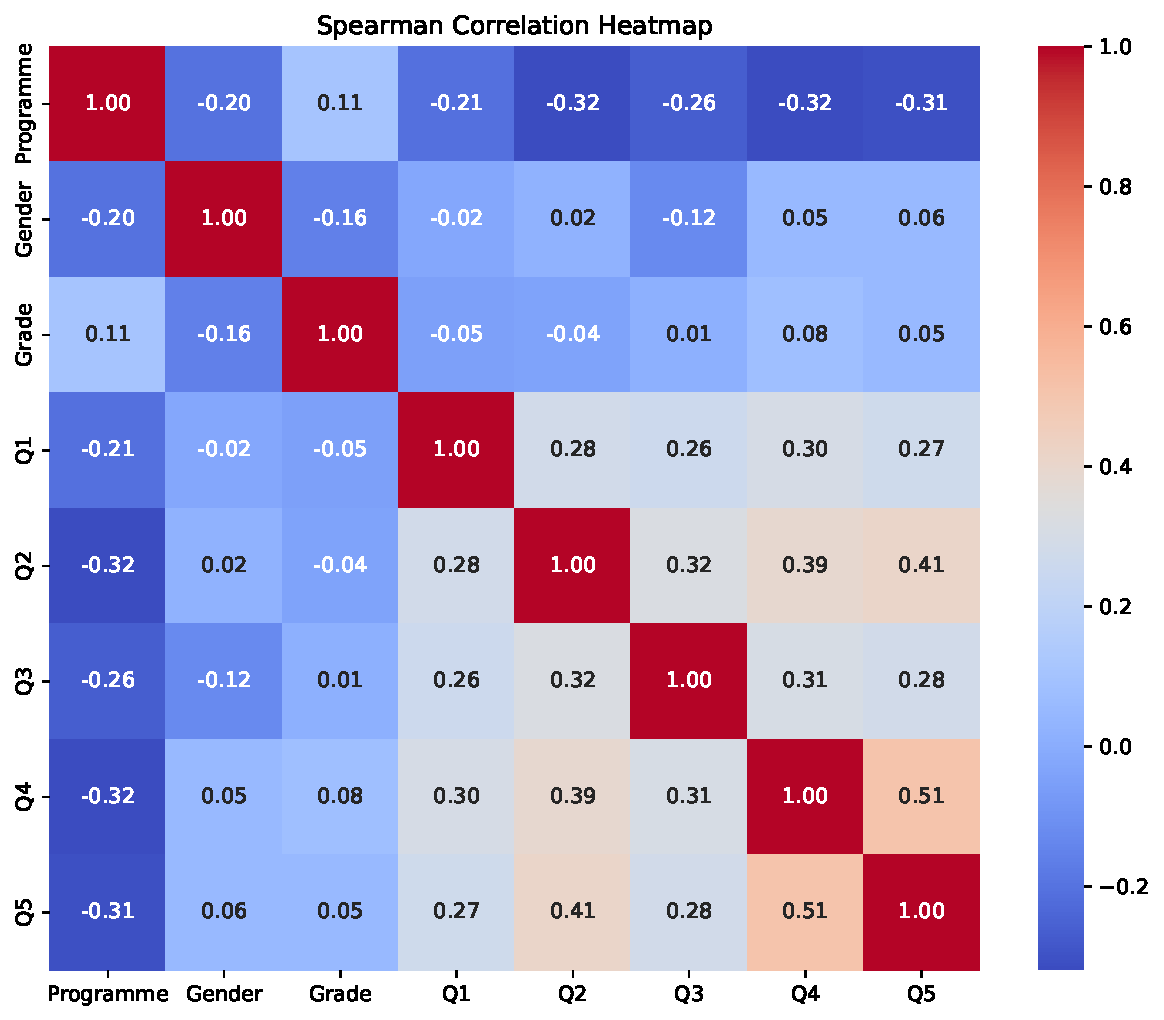
\includegraphics[width=0.5\linewidth]{fig/Task_1_0_Spearman.pdf}}
    \caption{Spearman correlation matrix}
    \label{fig:spearman}
\end{figure}
% 显然，对于 \textit{Programme}这一特征和其他特征几乎不具有相关性，因此需要对其他特征进行组合。此外，发现特征\textit{Q1}到\textit{Q5}具有一定的相关性，因此考虑将他们作为一个整体讨论。

Obviously, the feature of \textit{Programme} has almost \textbf{NO} correlation with other features. In addition, the features from \textit{Q1} to \textit{Q5} have a certain correlation, so it is deemed appropriate to conduct an integrated discussion of them as a unified entity.
% 此外，当选择的特征的时候可以考虑剔除 \textit{Gender} 因为他和 \textit{Programme} 负相关。
Additionally, when selecting features, consider \textbf{EXCLUDING} \textit{Gender} because it is negatively correlated with \textit{Programme}.
Now 3 method will be utilized to standardize the data.

%考虑到\textit{Q1},\textit{Q2},\textit{Q3},\textit{Q4},\textit{Q5}的分布可能具有离群性质，故采用 Robust 标准化标准化，使用中位数和四分位数间距代替均值和标准差。对异常值更鲁棒，能有效减少离群值对标准化结果的影响，其公式如下

Considering that the distributions of \textit{Q1}, \textit{Q2}, \textit{Q3}, \textit{Q4}, and \textit{Q5} may have outlier characteristics, \textbf{Robust} standardization is adopted. The median and interquartile range are used instead of the mean and standard deviation. It is more robust to outliers and can effectively reduce the impact of outliers on the standardization results. The formula is as follows. 
\begin{align}
x'=\dfrac{x-\text{median}(x)}{\text{IQR}(x)},\text{IQR}=Q_3(x)-Q_1(x)
\end{align}
%其中 Q_3(x) 和 Q_1(x) 分别代表特征 x 的第75百分位数和第25百分位数。
Where $Q_3(x)$ and $Q_1(x)$ represent the 75th percentile and the 25th percentile of the characteristic $x$, respectively.
The result see \textbf{Fig. \ref{fig:robust}}. As a result, 

\begin{figure}[h!]
    \centerline{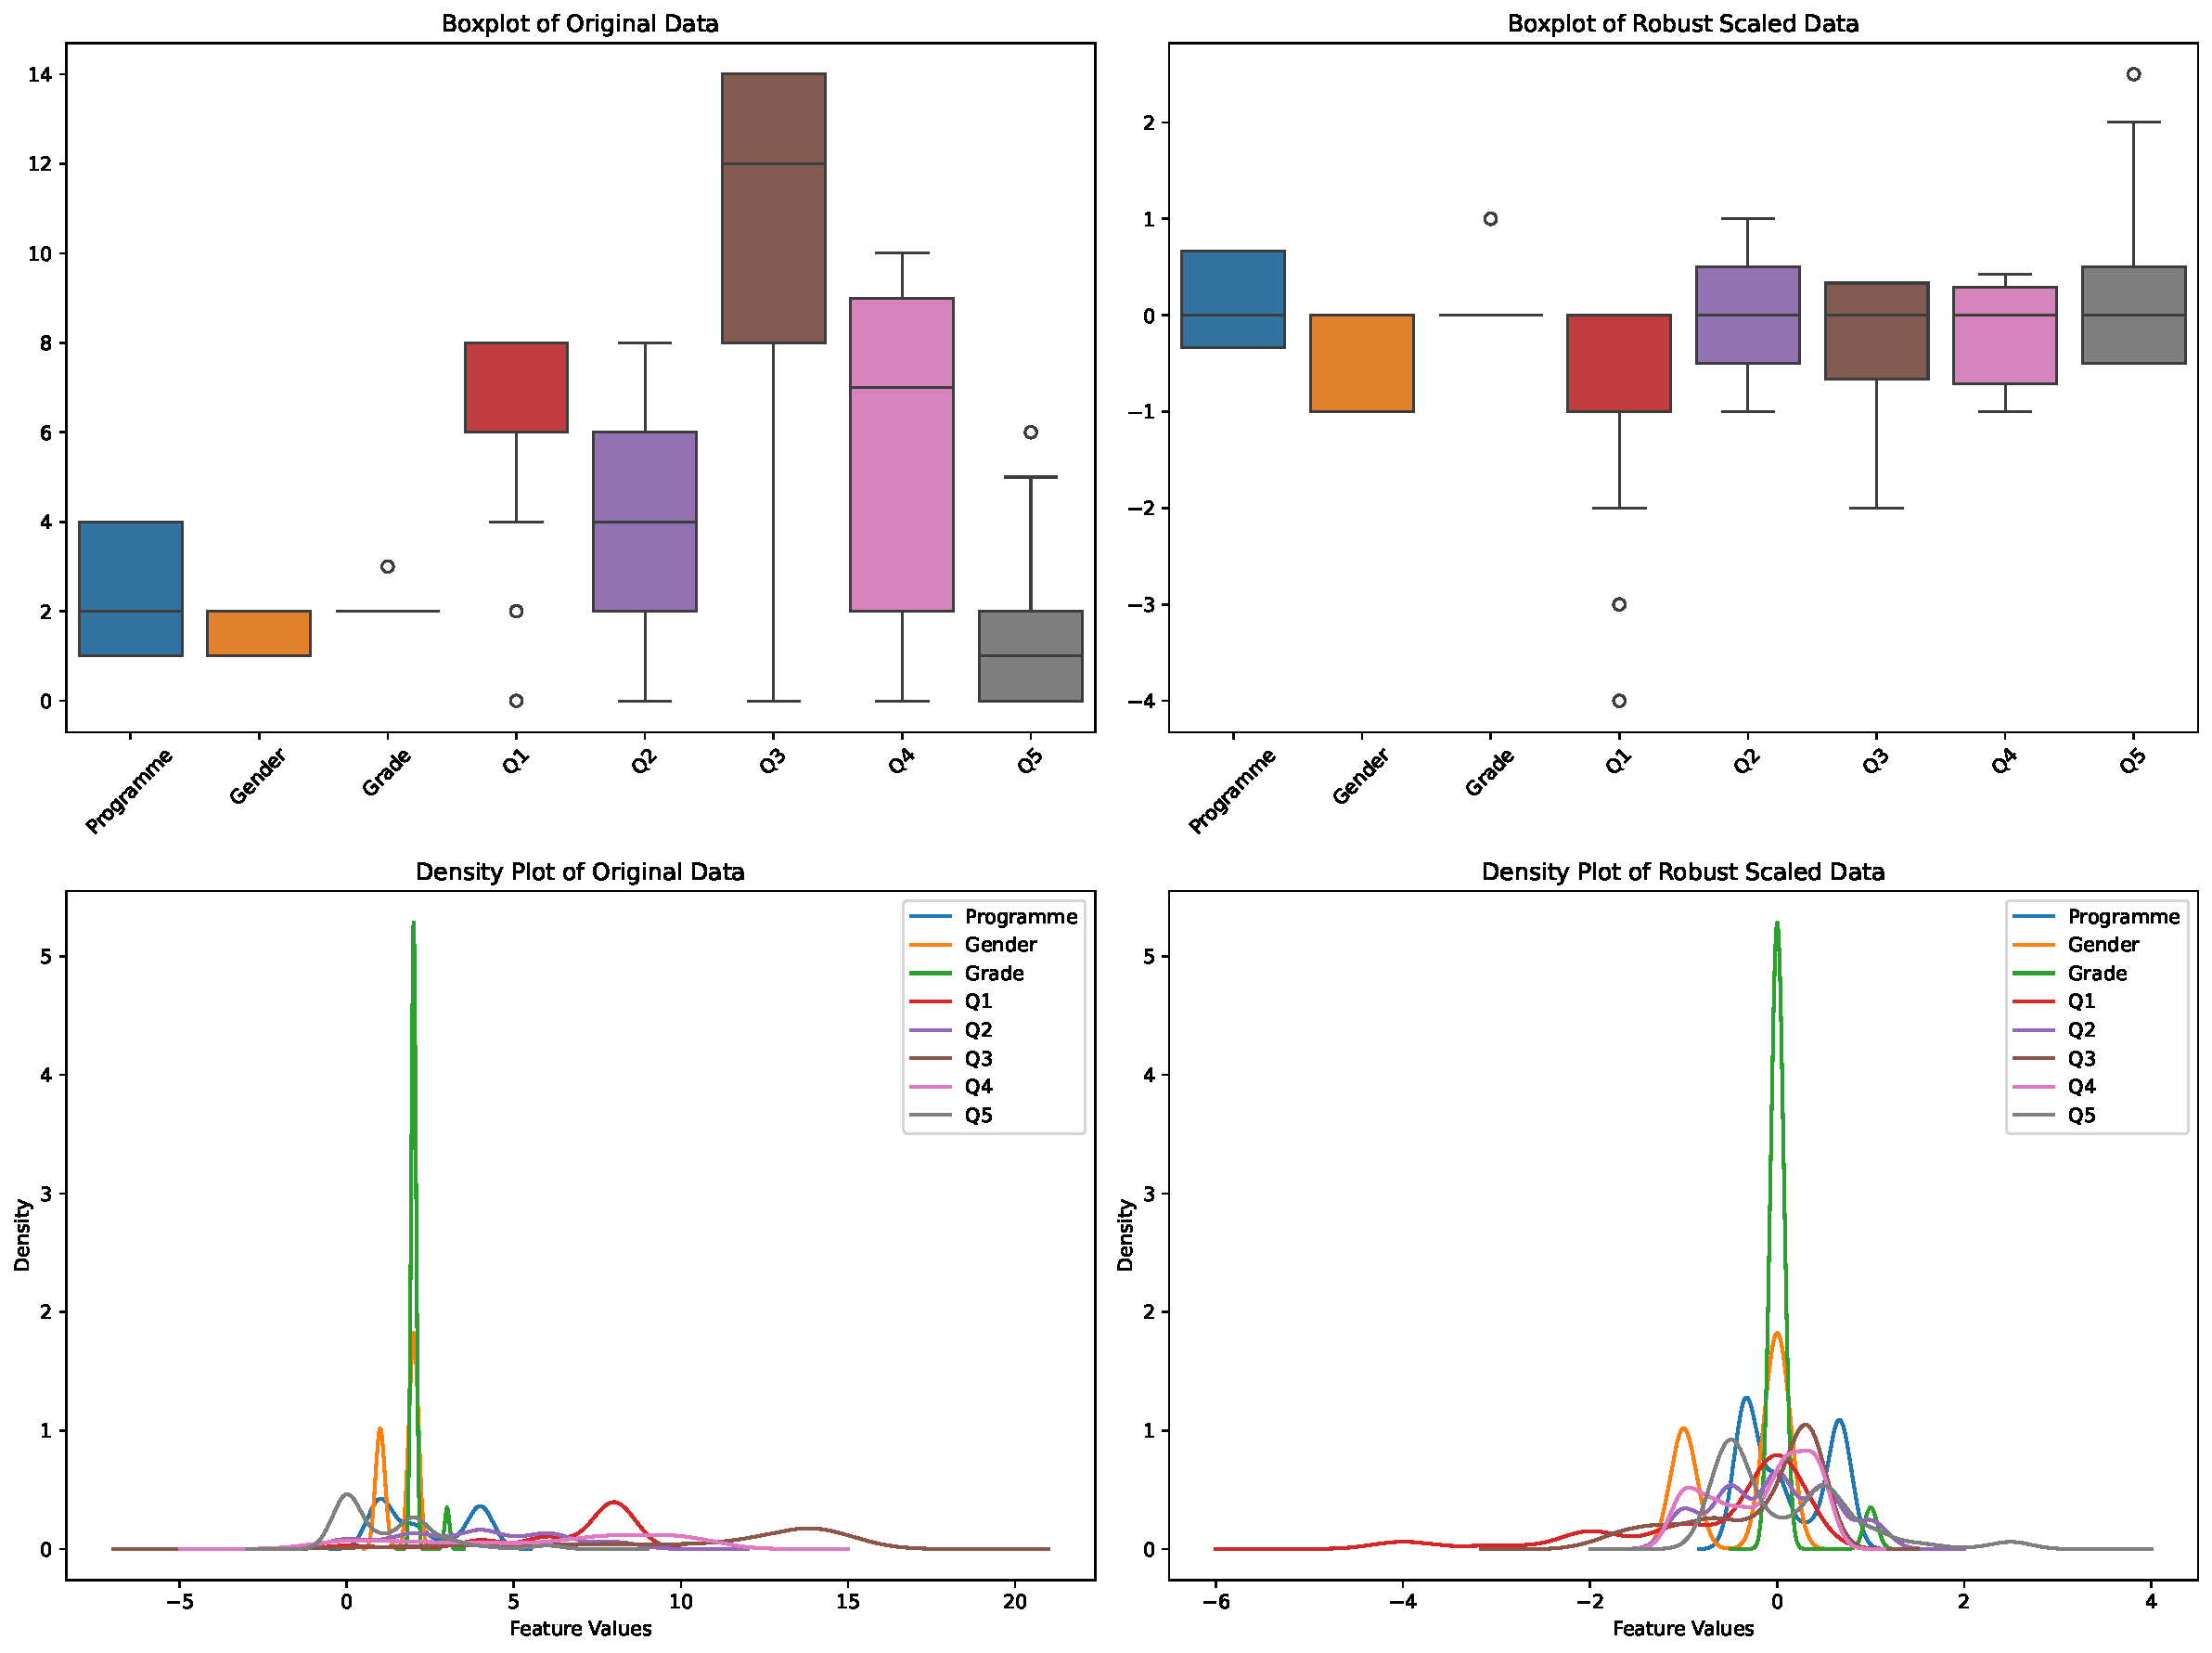
\includegraphics[width=1\linewidth]{fig/Task_1_1_Robust.pdf}}
    \caption{Robust standardization.}
    \label{fig:robust}
\end{figure}

% 不仅如此，采用Shapiro-Wilk 检查原始数据(\textit{Q1}到\text{Q5})是否符合正态分布来决定是否使用 z-score标准化，其指标$W$值如下
Moreover, the \textbf{Shapiro-Wilk Test} is employed to check whether the original data (from \textit{Q1} to \textit{Q5}) conforms to the normal distribution, which determined us whether to apply \textbf{Z-score} standardization. The value of $W$ indicates that closer to $1$ means better normality and vise versa.
\begin{align}
W=\dfrac{(\sum_{i-1}^{n}a_ix_{(i)})^2}{\sum_{i-1}^{n}(x_i-\overline{x})^2}
\end{align}

\begin{table}[h!]
    \centering
    \caption{Results of Shapiro-Wilk Normality Test for Features Q1 - Q5}
    \label{tab:shapiro_wilk_test}
    \begin{tabular}{lccccc}
        \toprule
        Feature & Original Statistic & Original p & Robust Statistic & Robust p \\
        \midrule
        Q1 & 0.6656 & 0.0000* & 0.6656 & 0.0000* \\
        Q2 & 0.9140 & 0.0000* & 0.9140 & 0.0000* \\
        Q3 & 0.7797 & 0.0000* & 0.7797 & 0.0000* \\
        Q4 & 0.8640 & 0.0000* & 0.8640 & 0.0000* \\
        Q5 & 0.7712 & 0.0000* & 0.7712 & 0.0000* \\
        \bottomrule
    \end{tabular}
    \vspace{0.5em}
    \begin{tablenotes}
        \item * Indicates significant deviation from normality at the $\alpha = 0.05$ level.
    \end{tablenotes}
\end{table}

% 假设 $\alpha = 0.05$，发现 对于 \textit{Q1} 到 \textit{Q5} 的p值均小于 $\alpha$因此拒绝原假设，不符合正态分布，因此不适用 Z-score 标准化方法。
Assuming $\alpha = 0.05$, it was found that the p-values for \textit{Q1} to \textit{Q5} are all less than $\alpha$.

Therefore, the null hypothesis is rejected, indicating that the data do \textbf{NOT} follow a normal distribution. Consequently, the Z-score standardization method is not applicable. 

% 从表格中\ref{tab:shapiro_wilk_test}可见数据严重偏态，因此可以先进行对数变换后再标准化。，见图 log
It can be seen from \textbf{Table \ref{tab:shapiro_wilk_test}} that the data is severely skewed. Therefore, a logarithmic transformation can be performed first, and then normalization. See \textbf{Fig. \ref{fig:log}}.

\begin{figure}[h!]
    \centerline{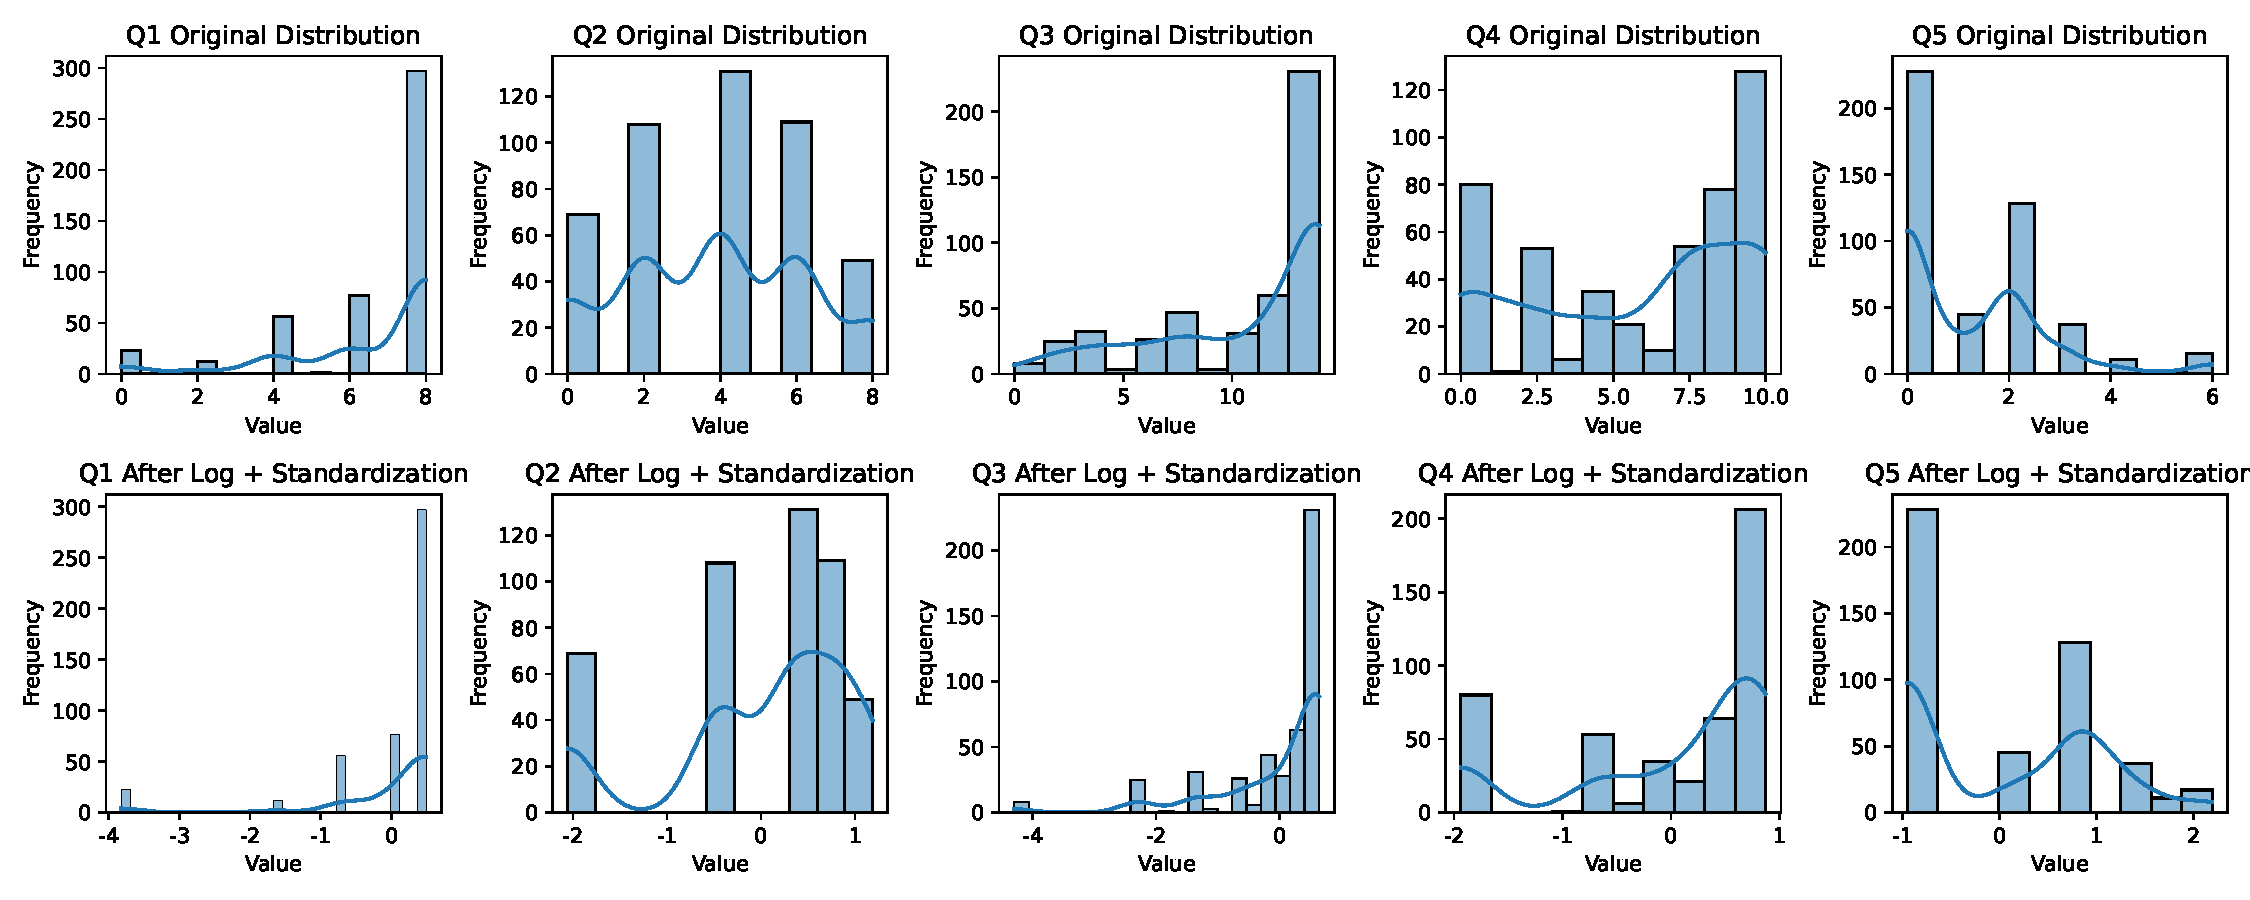
\includegraphics[width=1\linewidth]{fig/Task_1_3_Log.pdf}}
    \caption{Logarithmic standardization.}
    \label{fig:log}
\end{figure}

% 同样的，也可以使用 Box-Cox 变换法后进行标准化，见图 boxcox.
Similarly, using the Box-Cox transformation method followed by standardization. See \textbf{Fig. \ref{fig:boxcox}}.
\begin{figure}[h!]
    \centerline{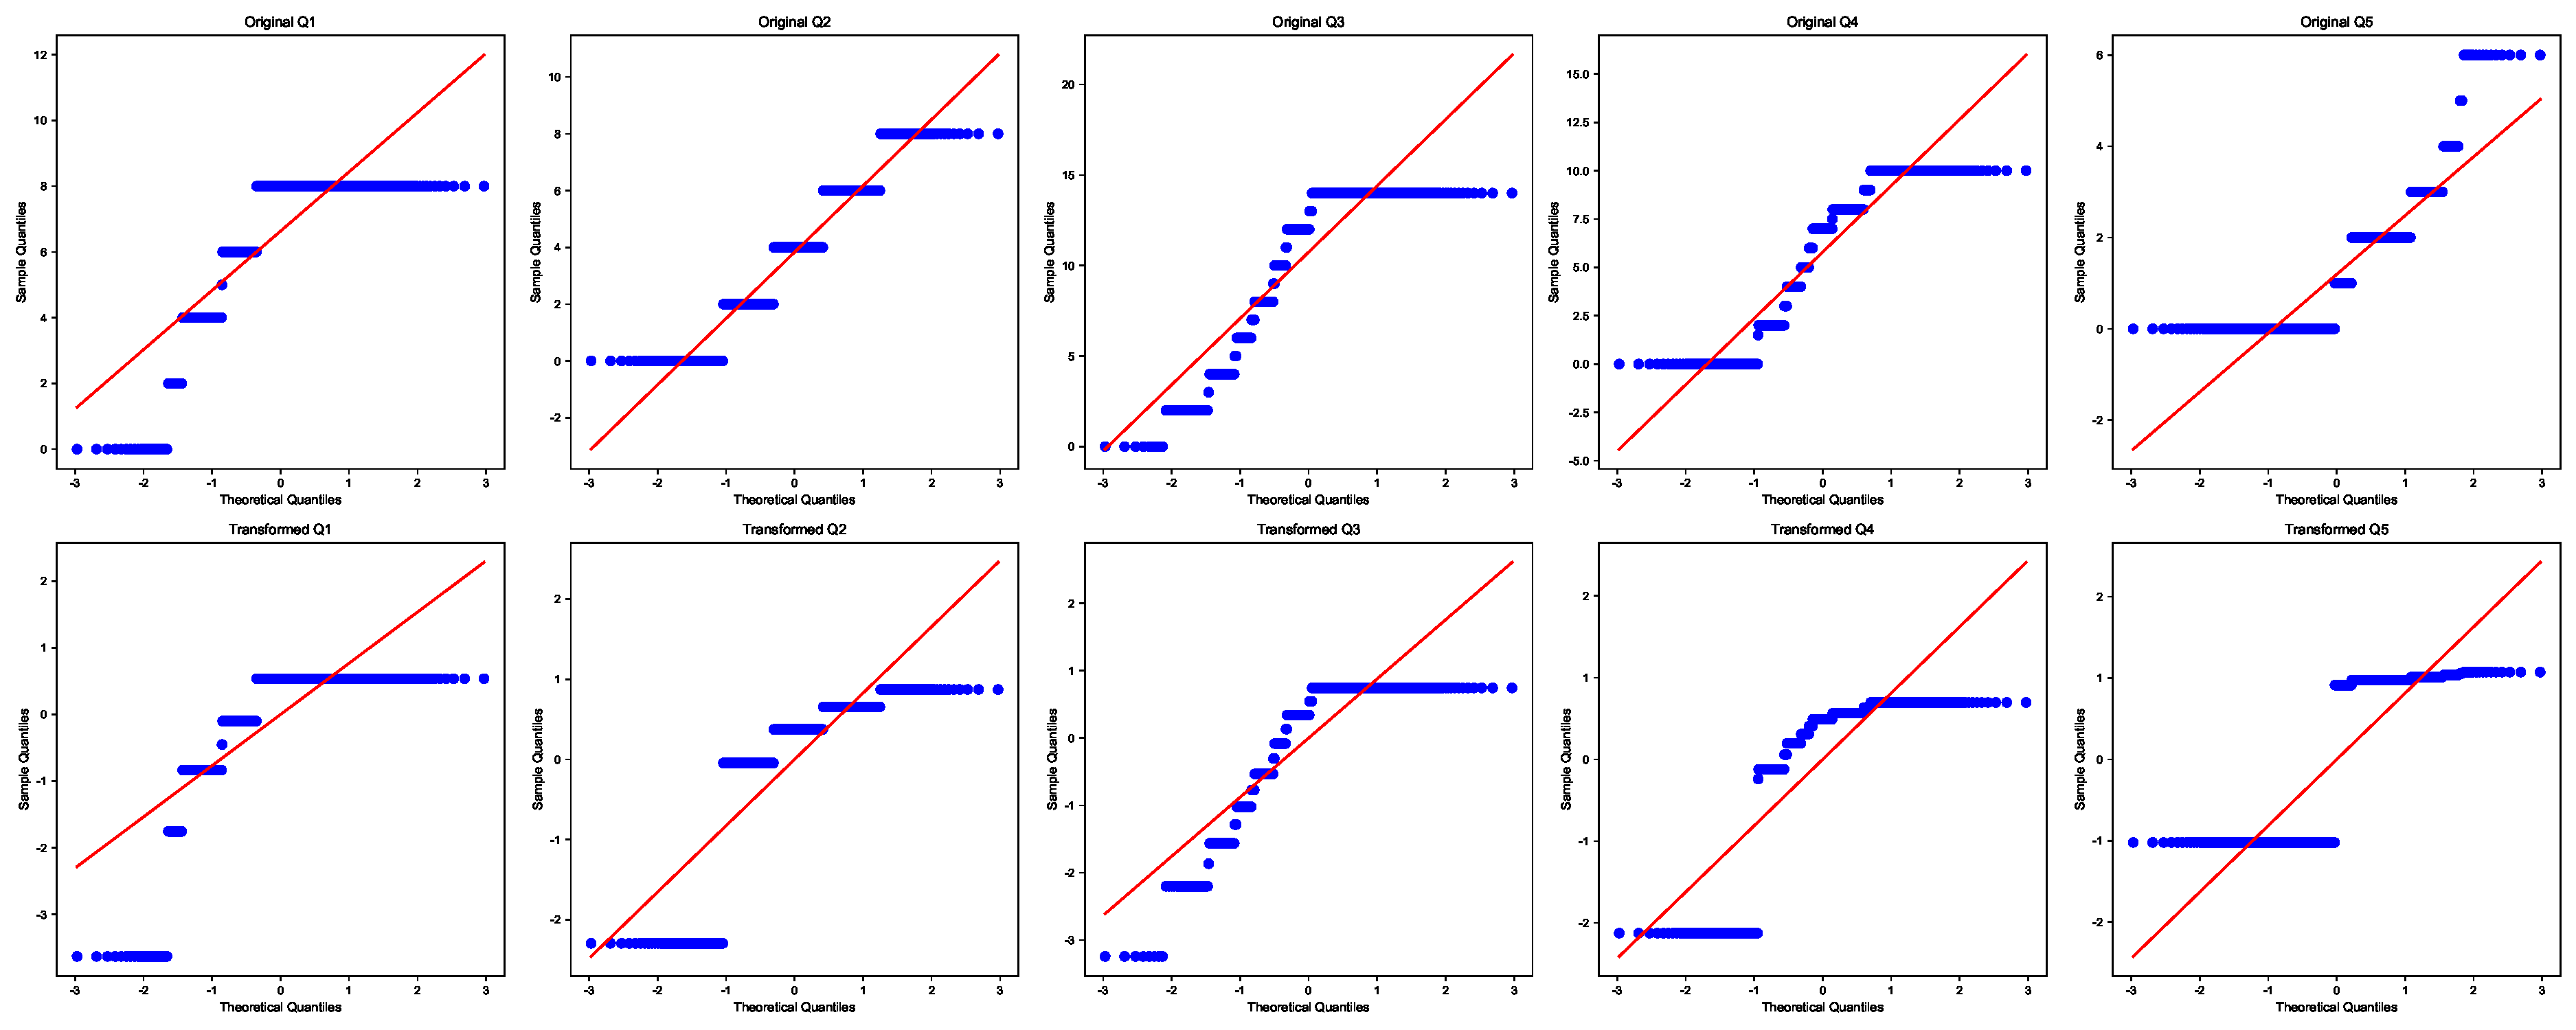
\includegraphics[width=1\linewidth]{fig/Task_1_4_BoxCox.pdf}}
    \caption{Box-Cox standardization.}
    \label{fig:boxcox}
\end{figure}

% 总而言之，对于数据标准化过程，使用了如下三种方法：
In general, for the data standardization process, the following 3 methods were used above: 
\begin{itemize}
    \item \textbf{Robust Standardization}, see \textbf{Fig. \ref{fig:robust}}.
    \item \textbf{Logarithmic Transformation + Normalization}, see \textbf{Fig. \ref{fig:log}}.
    \item \textbf{Box-Cox Transformation + Normalization}, see \textbf{Fig. \ref{fig:boxcox}}.
\end{itemize}

% 接下来通过均值和标准差这两个方法作为标准化的指标。评估方法如下：计算数据的每一个特征的均值、标准差后将结果取平均值。
% 显而易见的是，经过标准化后的数据均值接近0，标准差接近1，意味着标准化效果比原始数据更好
Next, use the \textbf{Mean} and \textbf{Standard Deviation} as indicators of standardization.
The evaluation method is as follows: calculate the mean and standard deviation for each feature of the data, and then take the average of the results. see the \textbf{Table \ref{tab:standardizeEvaluation}}. 

Obviously, after standardization, the mean of the data is close to 0 and the standard deviation is close to 1. In conclusion, the standardization effect is better than that of the original data. 
\begin{table}[h!]
    \centering
    \caption{Evaluation of Standardize}
    \label{tab:standardizeEvaluation}
    \begin{tabular}{lcccc}
        \toprule
        \multirow{2}{*}{\textbf{Statistic}} & \multicolumn{4}{c}{\textbf{Stanardize Method}} \\
       \cmidrule(lr){2-5}
        & \textbf{Original} & \textbf{Robust} & \textbf{Logarithmic} & \textbf{Box-Cox} \\
       \midrule
        Mean (\(\bar{x}\)) & 4.280 & -0.149 & 0.000 & 0.005 \\
        Standard Deviation (\(s\)) & 1.988 & 0.601 & 1.000 & 1.000 \\
        \bottomrule
        \end{tabular}
\end{table}

\section{\textbf{Task III:Clustering}}
% 本节聚类采用2种评估方法，分别是Davies  Bouldin Inde（DBI） 和Adjusted Rand Index（ARI）。其中DBI属于无真实标签的评估方法，而ARI属于带真实标签的评估方法
In this section, 2 evaluation methods are used for clustering, namely the \textbf{Davies Bouldin Index (DBI)} and the \textbf{Adjusted Rand Index (ARI)} \cite{hubert1985comparing}, \cite{davies2009cluster}.
Among them, DBI is an evaluation method without true labels, while ARI is an evaluation method with true labels. 

%调整兰德指数主要用于评估聚类结果与真实分类之间的相似度，取值范围在[−1,1]之间，值越高表示聚类结果与真实分类越相似。
The \textbf{ARI} is mainly used to evaluate the similarity between the clustering result and the true classification. Its value ranges $[-1,1]$. The higher the value, the more similar the clustering result is to the true classification. 

\begin{align}
    ARI=\dfrac{\sum_{i,j}\binom{n_{ij}}{2}-\dfrac{\left[\sum_{i}\binom{a_{i}}{2}\sum_{j}\binom{b_{j}}{2}\right]}{\binom{n}{2}}}{\dfrac{1}{2}\left[\sum_{i}\binom{a_{i}}{2}+\sum_{j}\binom{b_{j}}{2}\right]-\dfrac{\left[\sum_{i}\binom{a_{i}}{2}\sum_{j}\binom{b_{j}}{2}\right]}{\binom{n}{2}}}
\end{align}
\begin{table}[h!]
    \centering
    \caption{Notation Explanation of the ARI Formula}
    \begin{tabular}{ll}
        \toprule
        \textbf{Notation} & \textbf{Def.} \\
        \midrule
        $n$ & Total number of samples in the dataset \\
        $n_{ij}$ & Samples in $i$-th cluster of $C$ and $j$-th cluster of $K$ \\
        $a_i$ & Samples in $i$-th cluster of $C$ \\
        $b_j$ & Samples in $j$-th cluster of $K$ \\
        $\binom{n}{k}$ & Combination number, $\dfrac{n!}{k!(n - k)!}$ \\
        \bottomrule
    \end{tabular}
\end{table}
% DBI 通过计算簇内距离与簇间距离的比值来评估聚类结果，其公式如下

DBI evaluates the clustering result by calculating the ratio of the intra-cluster distance to the inter-cluster distance, and its formula is as follows.
\begin{align}
    DBI=\dfrac{1}{n}\sum_{i = 1}^{n}\max_{j\neq i}\left(\frac{S_{i}+S_{j}}{d_{ij}}\right)\\
    S_i = \dfrac{1}{\vert C_i\vert}\sum_{x\in C_i}d(x,c_i) 
\end{align}

\begin{table}[h!]
    \centering
    \caption{Notation in the DBI Formula}
        \begin{tabular}{ll}
            \toprule
         \textbf{Notation} & \textbf{Def.} \\
            \midrule
            $n$ & No. of clusters \\
            $S_i$ & Int. compactness of $i$-th cluster\\
            $C_i$ & Sample set of $i$-th cluster \\
            $c_i$ & Center of $i$-th cluster \\
            $d(x,c_i)$ & Dist. from sample $x$ to cluster center $c_i$ \\
            $d_{ij}$ & $d_{ij}=d(c_i,c_j)$ \\
            \bottomrule
        \end{tabular}
\end{table}

% 接下来对原始数据和三种标准化方法进行特征组合并使用主成分分析（PCA）进行降维。组合方法有很多，此处列举出一种，例如
Next, perform a feature combination on the original data and the 3 standardization methods and use Principal Component Analysis (PCA) for dimensionality reduction. There are many combination methods, and one of them is listed here. For example, 
\begin{itemize}
    \item Feature I: Grade + Q1 + Q2
    \item Feature II: Grade + Q3 + Q4
    \item Feature III: Grade + Q4 + Q5
\end{itemize}
% 之所以不选择 Programme 作为其中一个特征之一是因为 ARI 聚类要求给出实际标签，也就是Programme。并且根据 Fig. \ref{} 得出 Programme 几乎和其他的特征是负相关的。
% 此外不选择 Gender而选择Grade的原因是它与Programme负相关。
The reason for not selecting \textit{Programme} as one of the features is that when evaluating clustering using ARI, ground-truth labels are required—and \textit{Programme} itself serves as those labels. Additionally, as shown in \textbf{Fig. \ref{fig:spearman}}, \textit{Programme} is nearly negatively correlated with all other features.  
Furthermore, the reason for choosing \textit{Grade} over \textit{Gender} as a feature is that \textit{Gender} is negatively correlated with \textit{Programme} whereas \textit{Grade} shows the opposite (correlation with \textit{Programme}).
%对于这三组特征直接合并并使用PCA降维。结果见 Fig. \ref{fig:pcaComparation}.
Directly merge these 3 sets of features and perform dimensionality reduction using PCA. The results are shown in \textbf{Fig. \ref{fig:pcaComparation}}. 
\begin{figure}[h!]
    \centerline{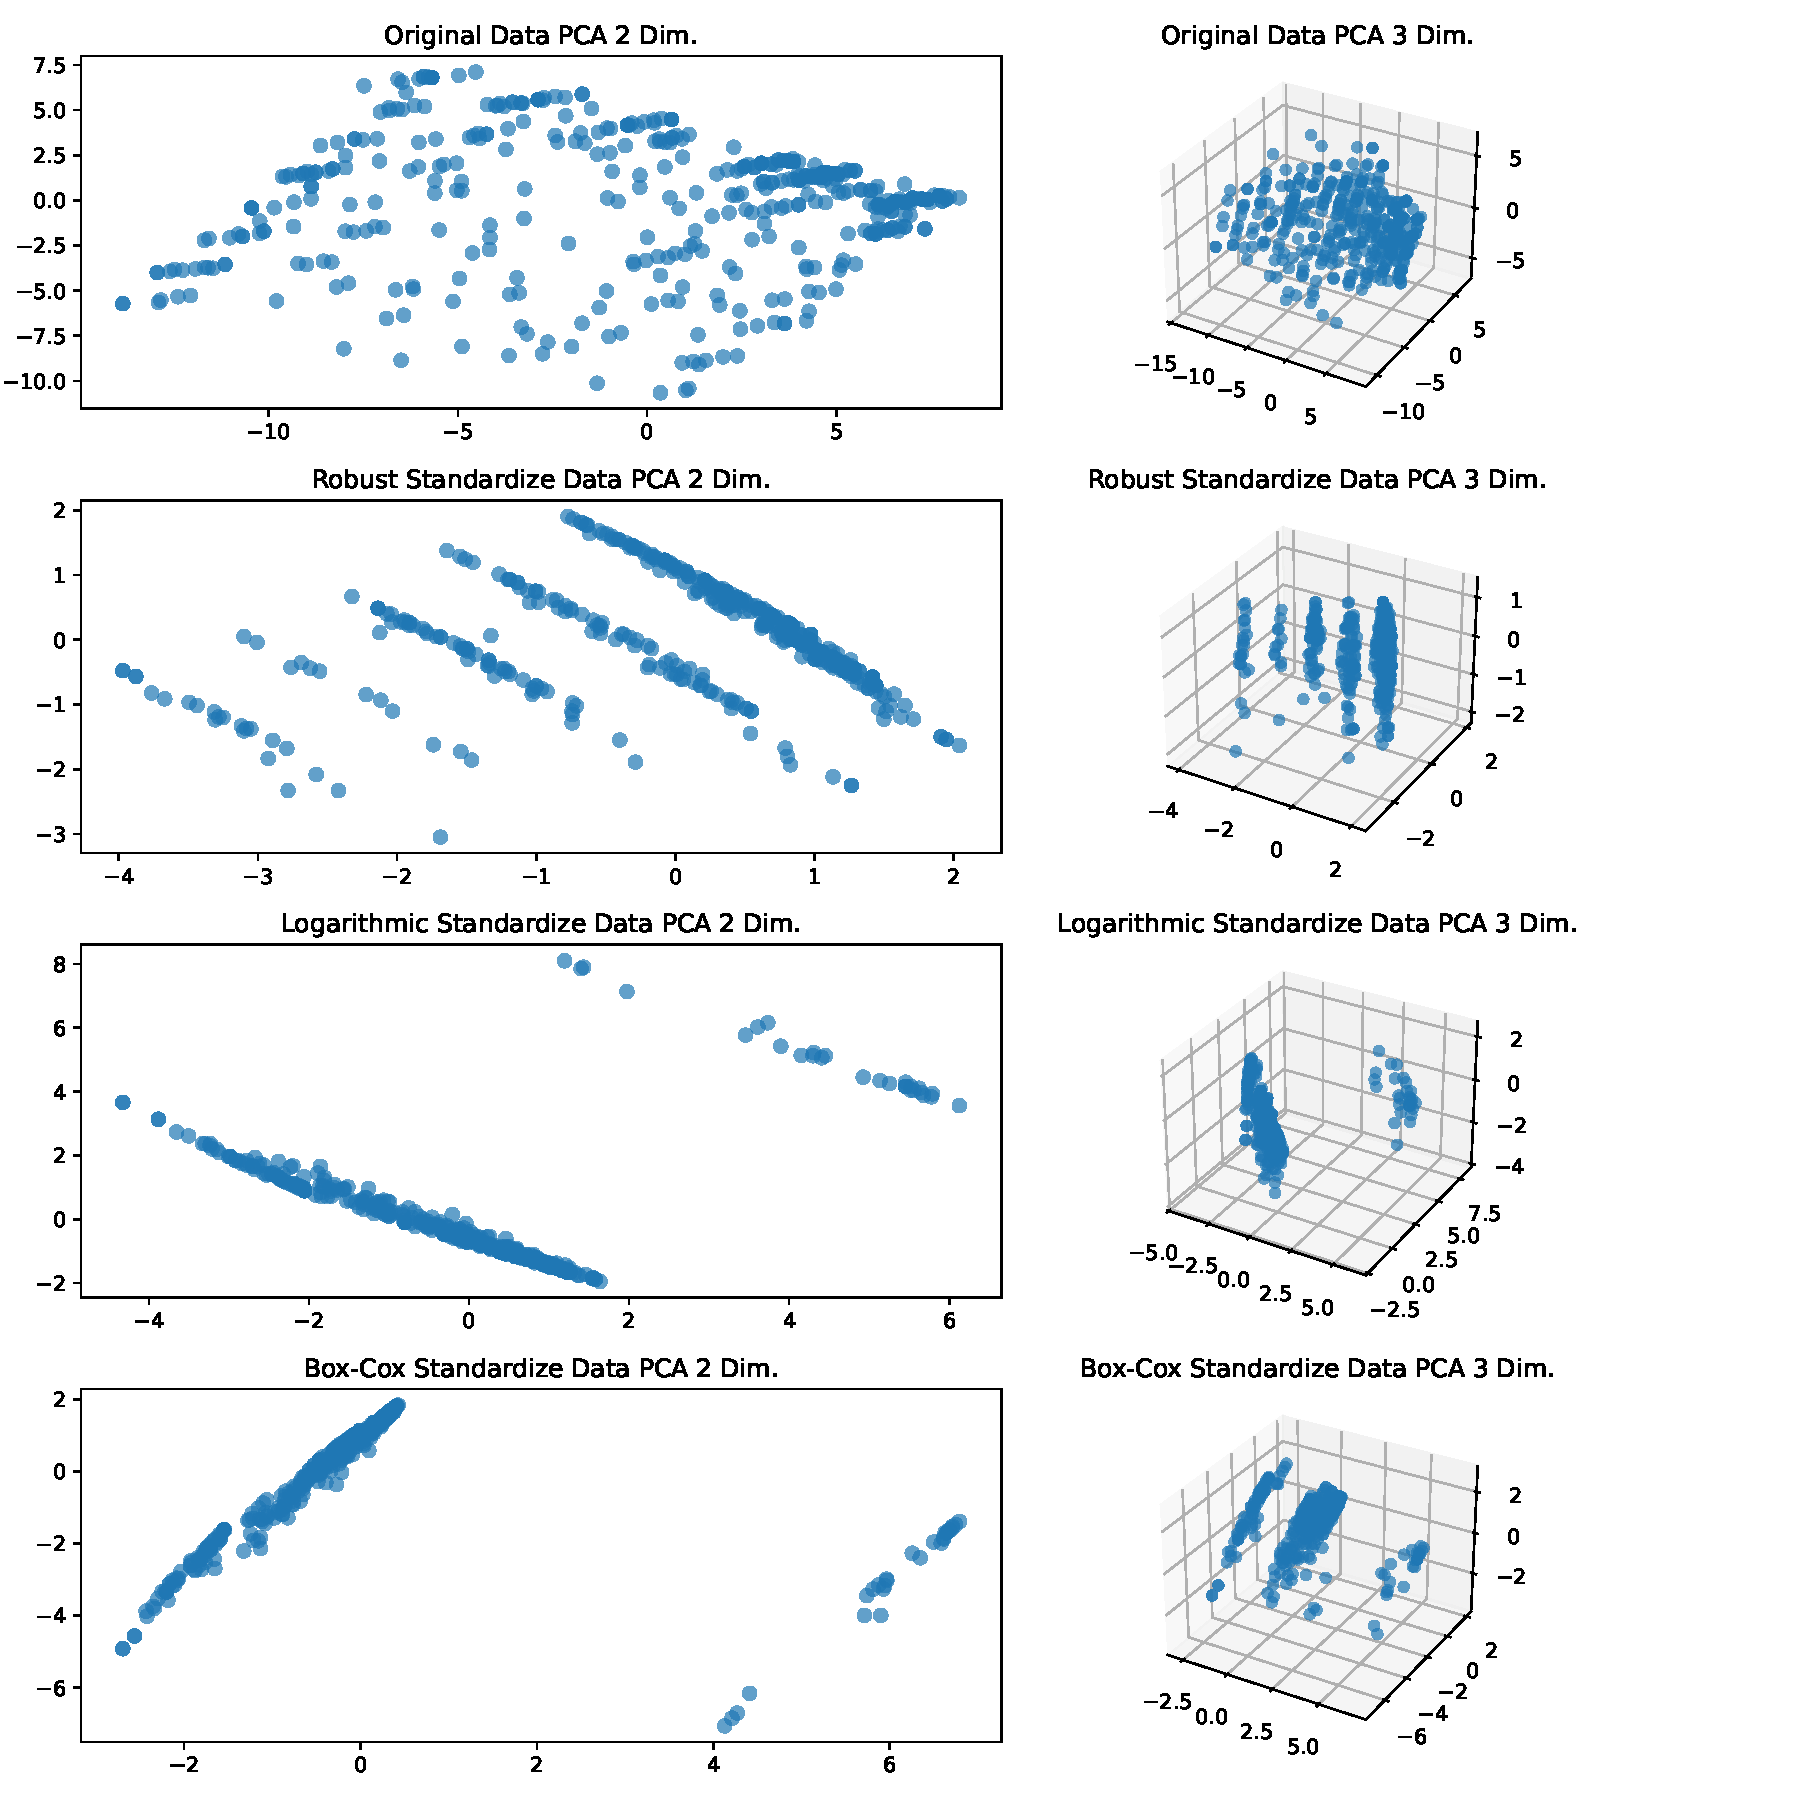
\includegraphics[width=0.75\linewidth]{fig/Task_3_0_PCA.pdf}}
    \caption{Dimension reduction to 2 \& 3 dim. using PCA}
    \label{fig:pcaComparation}
\end{figure}
% 接下来使用三种聚类方式，分别是 \textbf{K-Means},\textbf{DBSCAN} 以及\textbf{GMM}

Next, 3 clustering methods will be used, namely \textbf{K-Means}, \textbf{DBSCAN} and \textbf{GMM} clustering. 

% KMeans聚类结果如下，与原始数据相比，三种标准化后的数据明显优于原始数据：对ARI而言更接近1，说明处理后数据与真实标签一致性更高，对DBI而言更接近0证明聚类效果更好

The results of KMeans clustering are as follows: compared with the original data, the 3 standardized datasets significantly outperformed the original data. A value closer to 1 for ARI indicates higher consistency between the processed data and the ground-truth labels, while a value closer to 0 for DBI demonstrates better clustering performance in terms of compactness and separation.



\begin{table}[h!]
  \centering
  \begin{tabular}{ccc}
    \toprule
    & ARI & DBI \\
    \midrule
    Original Data KMeans val & 0.087 & 0.391 \\
    Robust Standardize KMeans & 0.099 & 0.337 \\
    Logarithmic Standardize KMeans val & 0.191 & 0.200 \\
    Box-Cox Standardize KMeans val& 0.181 & 0.193 \\
    \bottomrule
  \end{tabular}
  \caption{K-Means ARI \& DBI result}
  \label{tab:kmeans_ari_dbi}
\end{table}

\begin{figure}[h!]
  \centering
  \begin{tabular}{cc}
    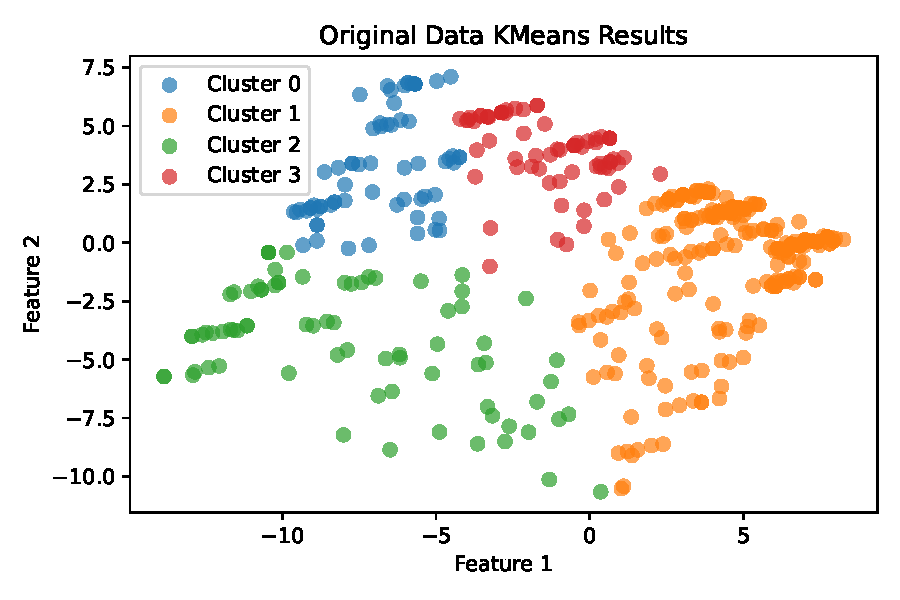
\includegraphics[width=0.22\textwidth]{fig/KMeans_image1.pdf} & 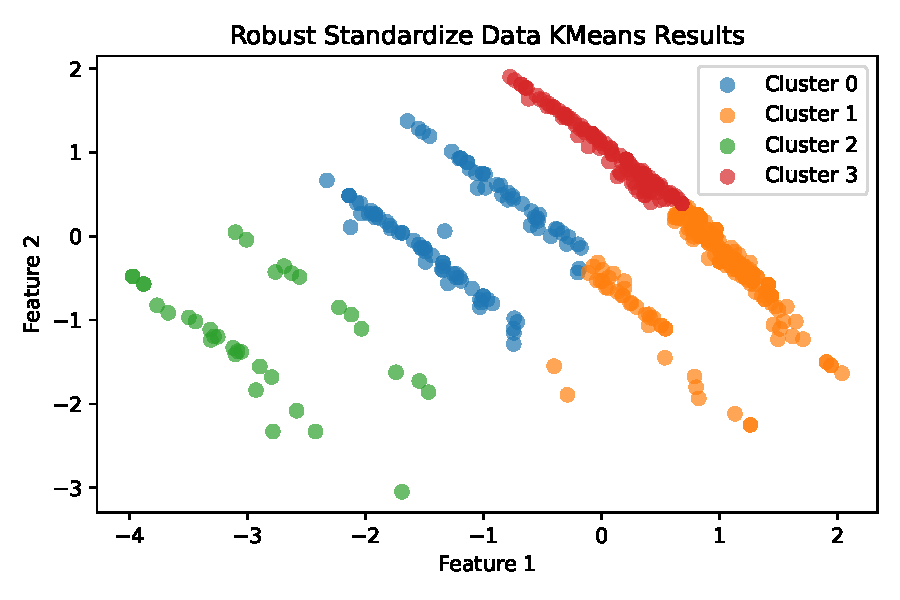
\includegraphics[width=0.22\textwidth]{fig/KMeans_image2.pdf} \\
    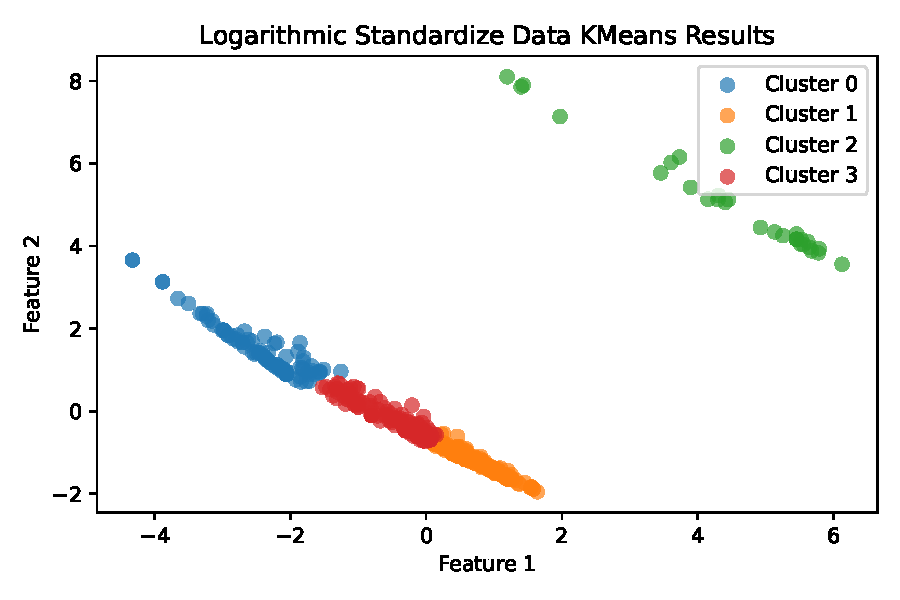
\includegraphics[width=0.22\textwidth]{fig/KMeans_image3.pdf} & 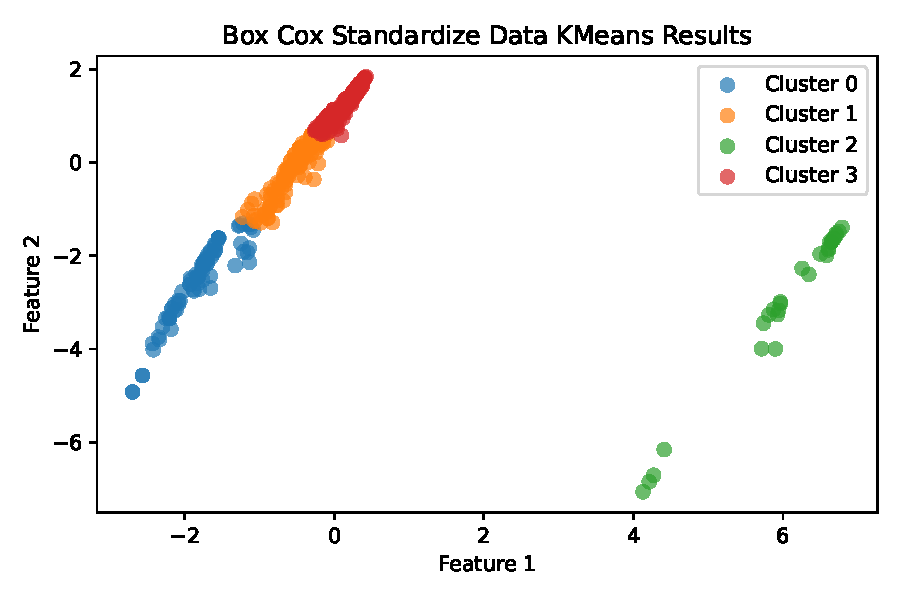
\includegraphics[width=0.22\textwidth]{fig/KMeans_image4.pdf} \\
  \end{tabular}
  \caption{K-Means cluster result}
  \label{fig:KMeansComparation}
\end{figure}


% 接下来，DBSCAN聚类。对于4组（原数据+3种变换数据）的DBSCAN聚类，采用调整eps的方式尽可能让他们聚为4类。
%结果如下


\begin{table}[h!]
  \centering
  \begin{tabular}{ccccc}
    \toprule
    Data Type& EPS & Min\_samples & ARI & DBI \\
    \midrule
     Original Data& 1.65 & 1 & 0.006 & 0.517 \\
     Robust Standardize& 0.70 & 1 & 0.037 & 0.367 \\
     Logarithmic Standardize& 0.80 & 1 & 0.106 & 0.190 \\
     Box-Cox Standardize& 0.60 & 1 & 0.104 & 0.128 \\
    \bottomrule
  \end{tabular}
  \caption{Parameters and ARI \& DBI result in DBSCAN}
  \label{tab:DBSCAN_ARI_DBI}
\end{table}

\begin{figure}[h!]
  \centering
  \begin{tabular}{cc}
    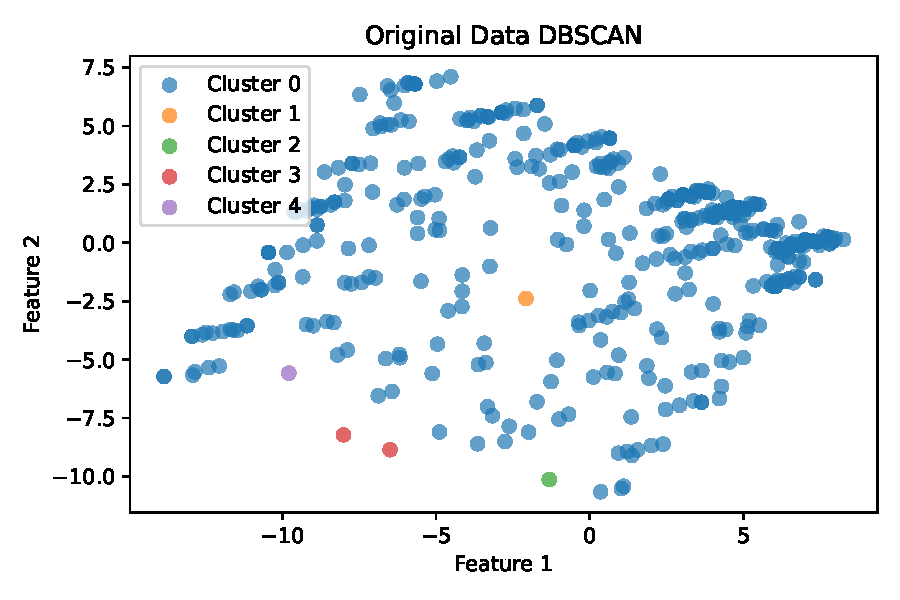
\includegraphics[width=0.22\textwidth]{fig/DBSCAN_image1.pdf} & 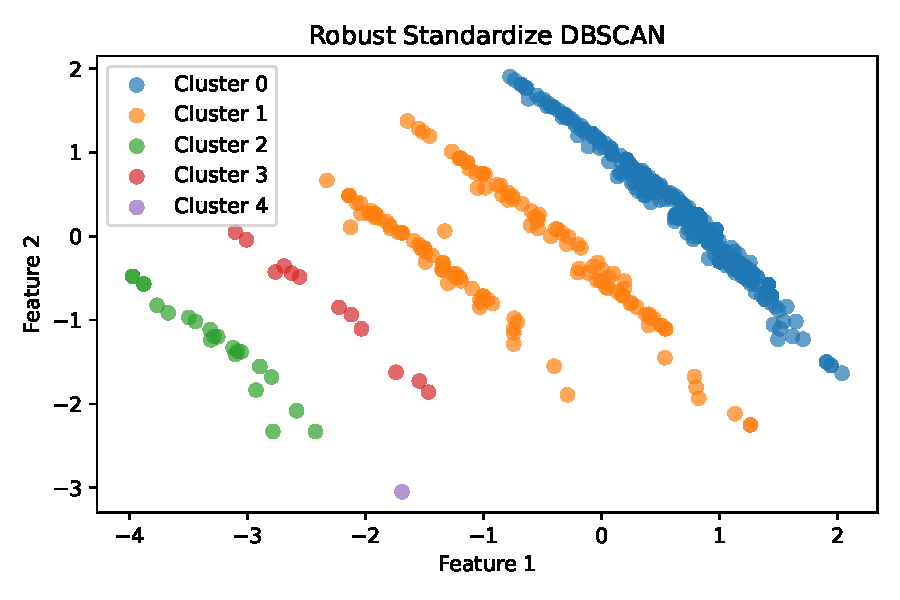
\includegraphics[width=0.22\textwidth]{fig/DBSCAN_image2.pdf} \\
    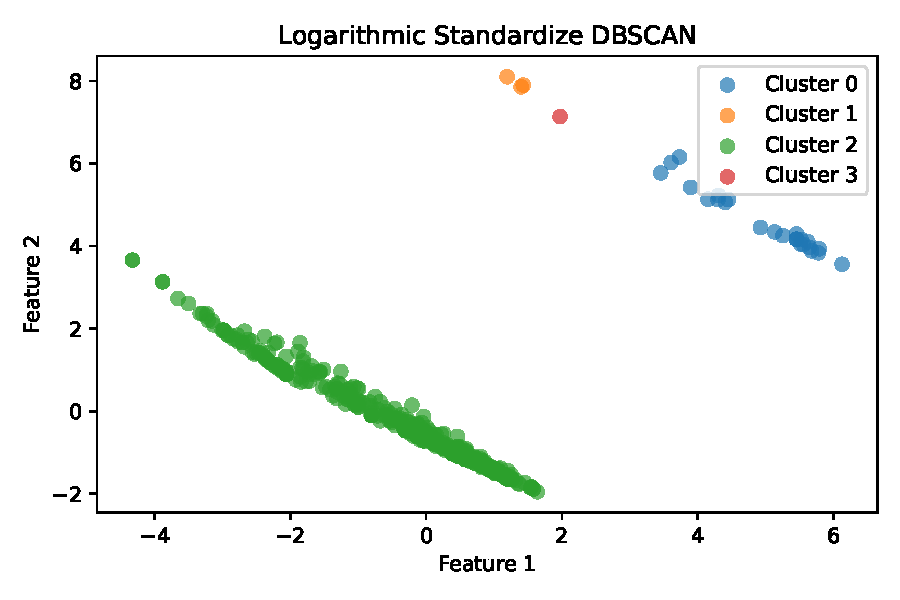
\includegraphics[width=0.22\textwidth]{fig/DBSCAN_image3.pdf} & 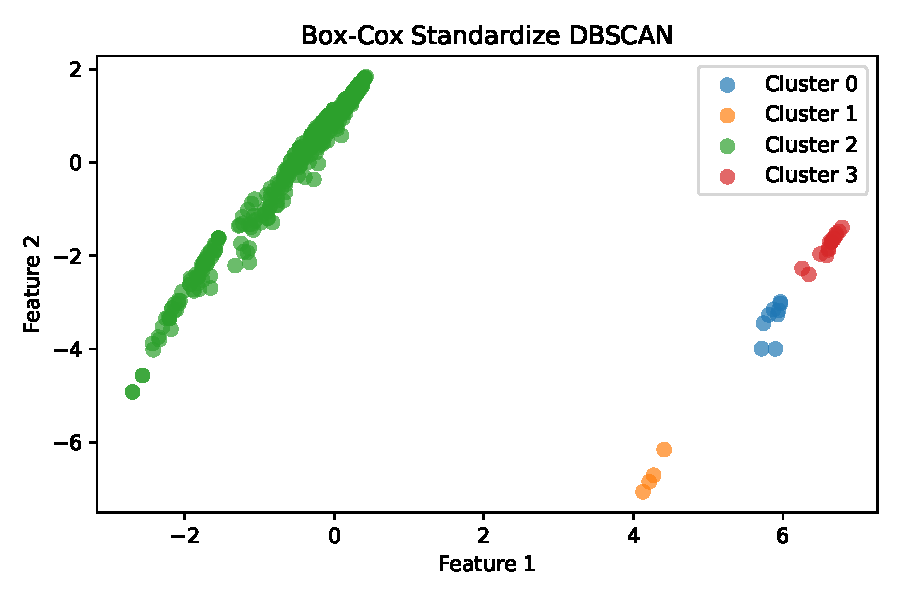
\includegraphics[width=0.22\textwidth]{fig/DBSCAN_image4.pdf} \\
  \end{tabular}
  \caption{DBSCAN cluster result}
  \label{fig:DBScanComparation}
\end{figure}

% 显然DBSCAN对于原始未处理的数据完全不友好，而对于执行了三种不同变化的数据友好。同时，ARI均比原始数据高，意味着更符合实际分类，而DBI均比原始数据低，意味着聚类模型更优秀。
Clearly, DBSCAN is less effective on raw, unprocessed data but performs better on data that has undergone 3 different transformations. The ARI values for the transformed data are higher than those for the original data, indicating a closer match with the actual classification. Furthermore, the DBI values for the transformed data are all lower than those for the original data, suggesting that the clustering models built from the transformed data are more optimal. See \textbf{Fig. \ref{fig:DBScanComparation}} and \textbf{table \ref{tab:DBSCAN_ARI_DBI}}.

% 接下来使用高斯混合(GMM)聚类，选择n_components=4，结果如下
Next, we use Gaussian Mixture Model (GMM) clustering with n\_components=4, and the results are as follows.

\begin{table}[h!]
  \centering
  \begin{tabular}{ccc}
    \toprule
    Data Type& ARI & DBI \\
    \midrule
     Original Data& 0.086 & 0.397 \\
     Robust Standardize & 0.050 & 0.388 \\
     Logarithmic Standardize& 0.206 & 0.151 \\
     Box-Cox Standardize& 0.147 & 0.189 \\
    \bottomrule
  \end{tabular}
  \caption{GMM ARI \& DBI result}
  \label{tab:GMM_ARI_DBI}
\end{table}

\begin{figure}[h!]
  \centering
  \begin{tabular}{cc}
    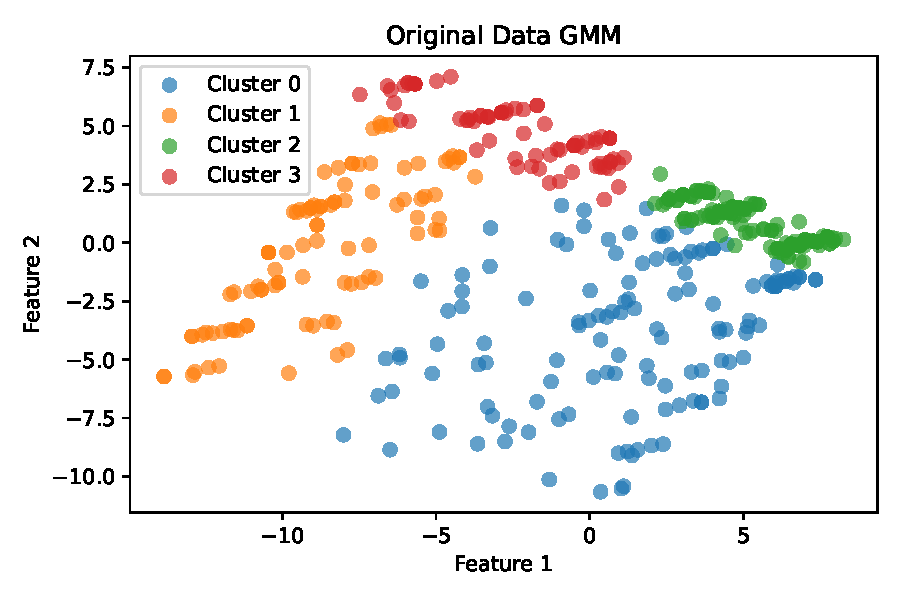
\includegraphics[width=0.22\textwidth]{fig/GMM_image1.pdf} & 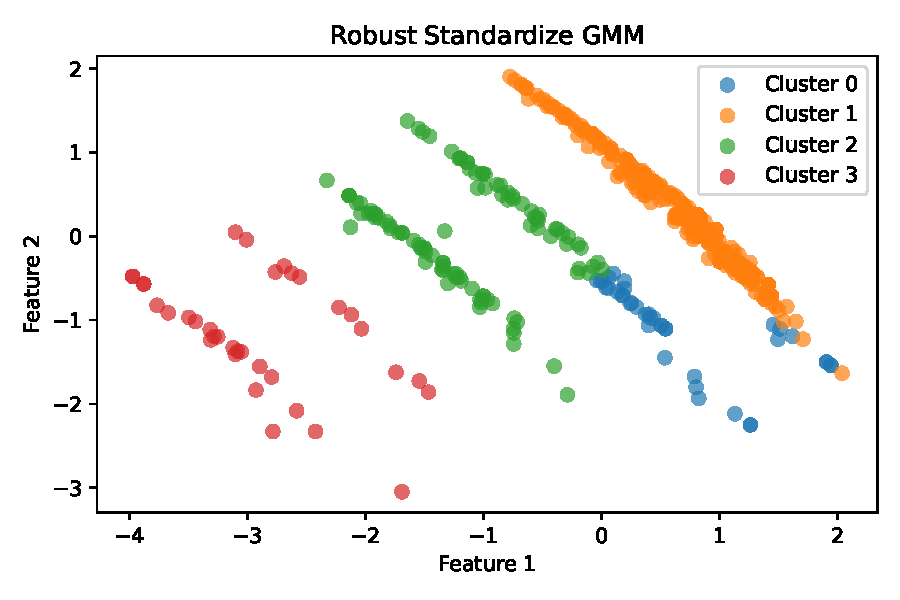
\includegraphics[width=0.22\textwidth]{fig/GMM_image2.pdf} \\
    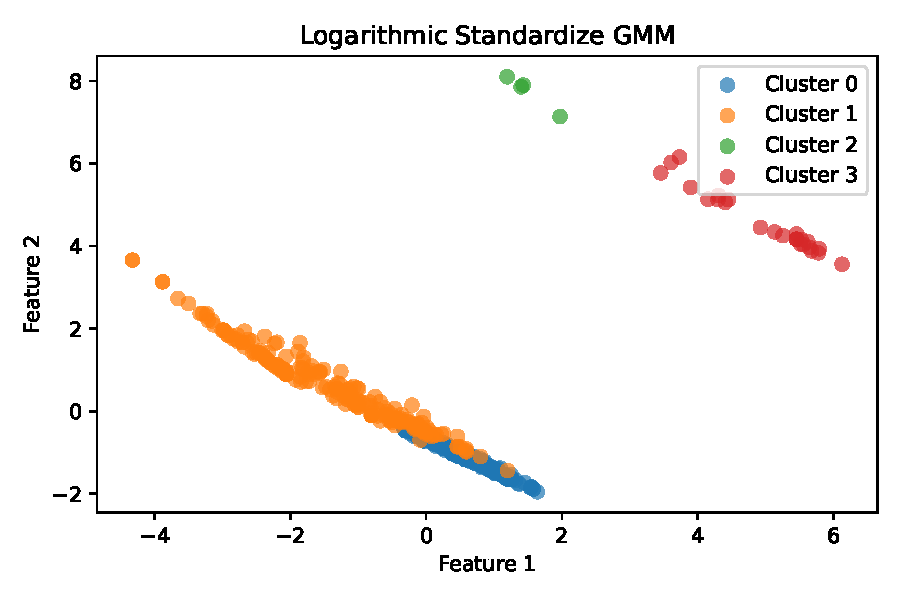
\includegraphics[width=0.22\textwidth]{fig/GMM_image3.pdf} & 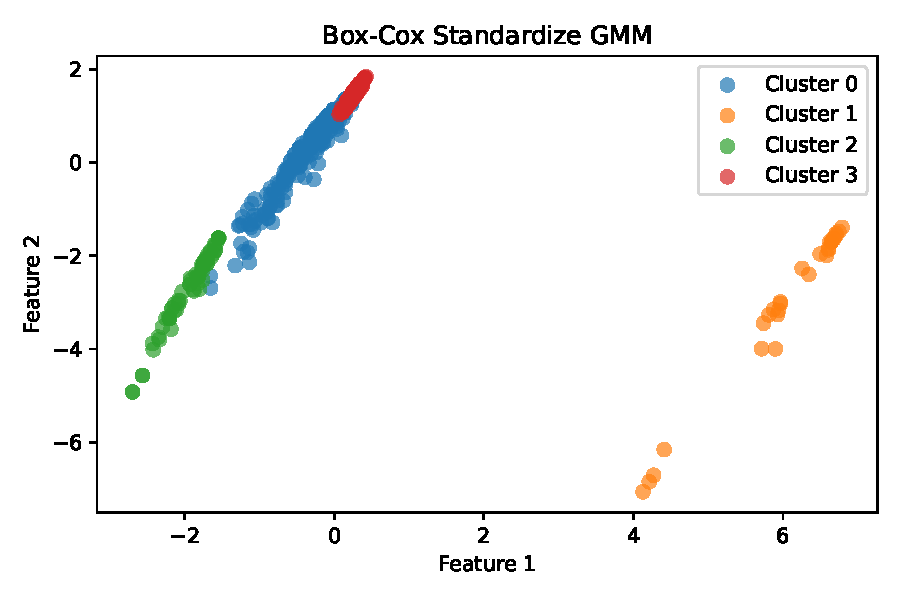
\includegraphics[width=0.22\textwidth]{fig/GMM_image4.pdf} \\
  \end{tabular}
  \caption{GMM cluster result}
  \label{fig:GMMComparation}
\end{figure}

\section{\textbf{Task IV: Classification}}
%在本节中会用到三种分类器，分别属于传统机器学习分类器--逻辑回归（Logistic Regression）、集成学习分类器--Boosting 类模型和深度学习分类器人工神经网络（ANN）
In this section, we will attempt to use 3 different classifiers, which respectively belong to: 
\begin{itemize}
    \item Traditional machine learning classifiers—Logistic Regression
    \item Ensemble learning classifiers—Boosting-based models
    \item Deep learning classifiers—Artificial Neural Network (ANN)
\end{itemize}
% 此外训练集和测试集的划分为8:2，随机选取。
Additionally, the training and test sets are split into an 7:3 ratio through random selection.
% 相比于聚类分析，分类预测选择应当添加更多的数据来完善模型，具体而言就是使用更多组特征组合，本节种三个模型的数据选择如下：

Compared to cluster analysis, classification prediction should incorporate more data to refine the model—specifically by using more sets of feature combinations. The data selection for the three models in this section is as follows:

\begin{table}[h!]
    \centering
    \caption{Feature combination}
    \begin{tabular}{ll}
        \toprule
        \textbf{Combination No.} & \textbf{Features} \\
        \midrule
        1 & \textit{Q1}, \textit{Q2}, \textit{Q3}, \textit{Q4}, \textit{Q5} \\
        2 & \textit{Grade}, \textit{Gender}\\
        3 & \textit{Q1}, \textit{Q3}\\
        4 & \textit{Q2}, \textit{Q4}\\
        5 & \textit{Q3}, \textit{Q5}\\
        6 & \textit{Q1}, \textit{Q2}, \textit{Q3}\\
        7 & \textit{Q2}, \textit{Q3}, \textit{Q4}\\
        8 & \textit{Q3}, \textit{Q4}, \textit{Q5}\\
        9 & \textit{Q4}, \textit{Q5}\\
        10 & \textit{Q1}, \textit{Q5}\\
        11 & \textit{Q1}, \textit{Q2}\\
        \bottomrule
    \end{tabular}
\end{table}

% 这些组合将会同样进行3种变换(Section I种的3种)分别是...Robust Standardize, Logarithmic Standardize 以及 Box-Cox Standardize,
% 随后使用PCA降维到1维然后合并为一个具有11个特征的矩阵，作为模型的传入，并且模型需要传出4个结果代表所预测的专业。最终的结果是:

These combinations will also undergo 3 types of transformations (mentioned in Section II), specifically: \textbf{Robust Standardization}, \textbf{Logarithmic Standardization}, and \textbf{Box-Cox Standardization}. Subsequently, PCA will be used to reduce dimensionality to 1 dimension, which will then be merged into a matrix with 11 features to serve as input for the model. Additionally, the model is required to output four results representing the predicted \textit{Programme}. The final result of accuracy is:
\begin{table}[h!]
    \centering
    \caption{Accuracy for Different Classifier under Different Transformation}
    \begin{tabular}{lllll}
        \toprule
        \textbf{Classifier $\setminus$ Trans.} & \textbf{Original}& \textbf{Robust}& \textbf{Logarithmic}& \textbf{Box-Cox} \\
        \midrule
        Logistic Regression & 52.85\%	&53.57\%&	\textbf{\color{red}{60.71\%}}&	59.28\%\\
        Boosting-based & \textbf{\color{red}{65.00\%}}&	58.57\%&	58.57\%&	62.85\%\\
        Transformer & 57.85\%	&52.14\%	&58.57\%&	$\color{red}\textbf{64.28\%}$\\
        \bottomrule
    \end{tabular}
    \label{fig:accuracyResult}
\end{table}

% 对于Logistic Regression Classifier模型(LR)模型而言，经过3种transformations后的数据明显准确率更高，最高准确率的数据使用了Logarithmic标准化，因此可以认为对于传统的分类模型（LR）而言，数据预处理是有必要的，可以在一定程度上提高模型的识别率。由 Fig. \ref{fig:2x2ConfusionMatrixLRClassifier} 可知LR classifier 把专业D错误地分类为专业A的情况十分常见。

Regarding the Logistic Regression Classifier (LR) model: the data processed through the three transformations demonstrated significantly higher accuracy. The dataset with the highest accuracy utilized Logarithmic Standardization. Therefore, it can be concluded that data preprocessing is necessary for traditional classification models (LR) and can, to a certain extent, improve the model's recognition rate. As shown in \textbf{Fig. \ref{fig:2x2ConfusionMatrixLRClassifier}}, the LR classifier frequently misclassifies \textit{Programme} D as \textit{Programme} A wrongly.

\begin{figure}[h!]
  \centering
  \begin{minipage}{0.22\textwidth}
    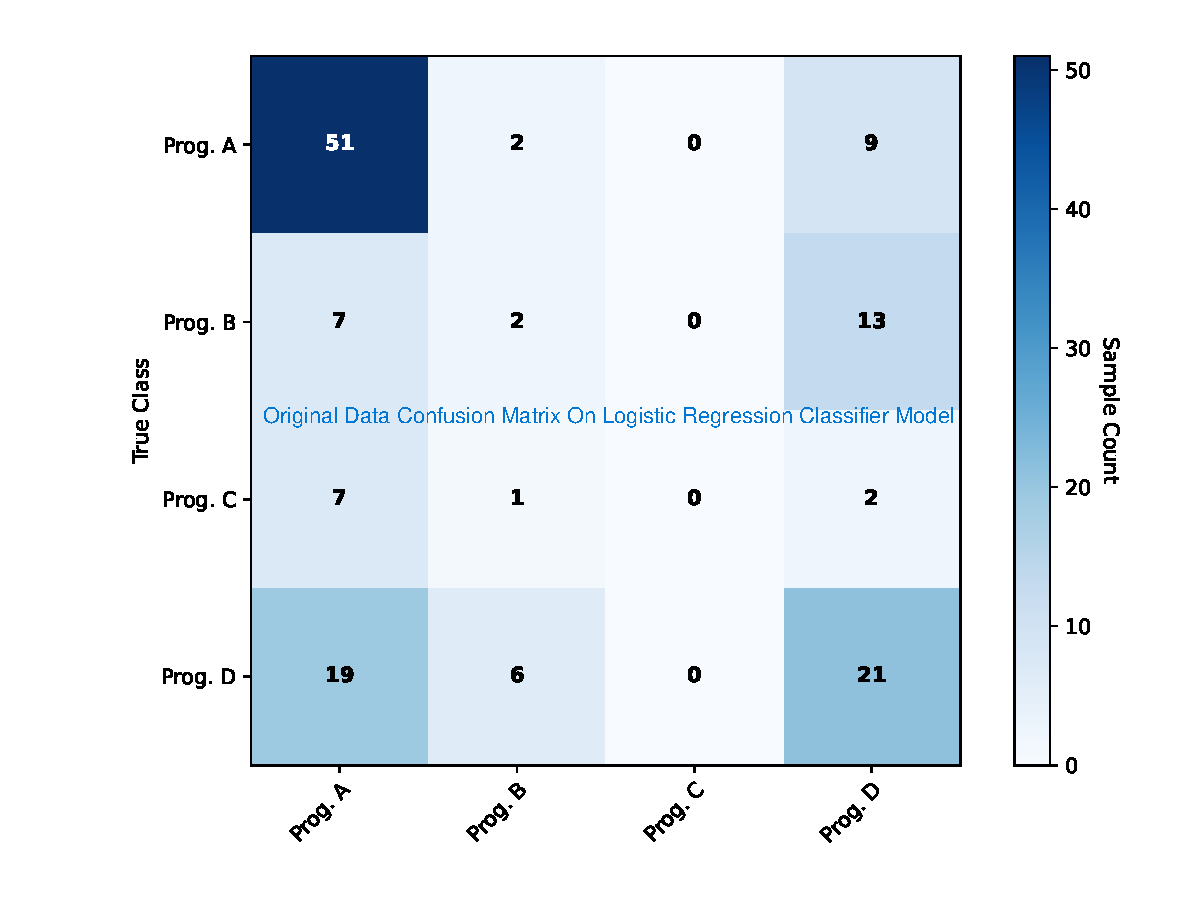
\includegraphics[width=\linewidth]{fig/RAW_ConfusionMatrix_1.pdf}
    \caption{Original}
  \end{minipage}%
  \begin{minipage}{0.22\textwidth}
    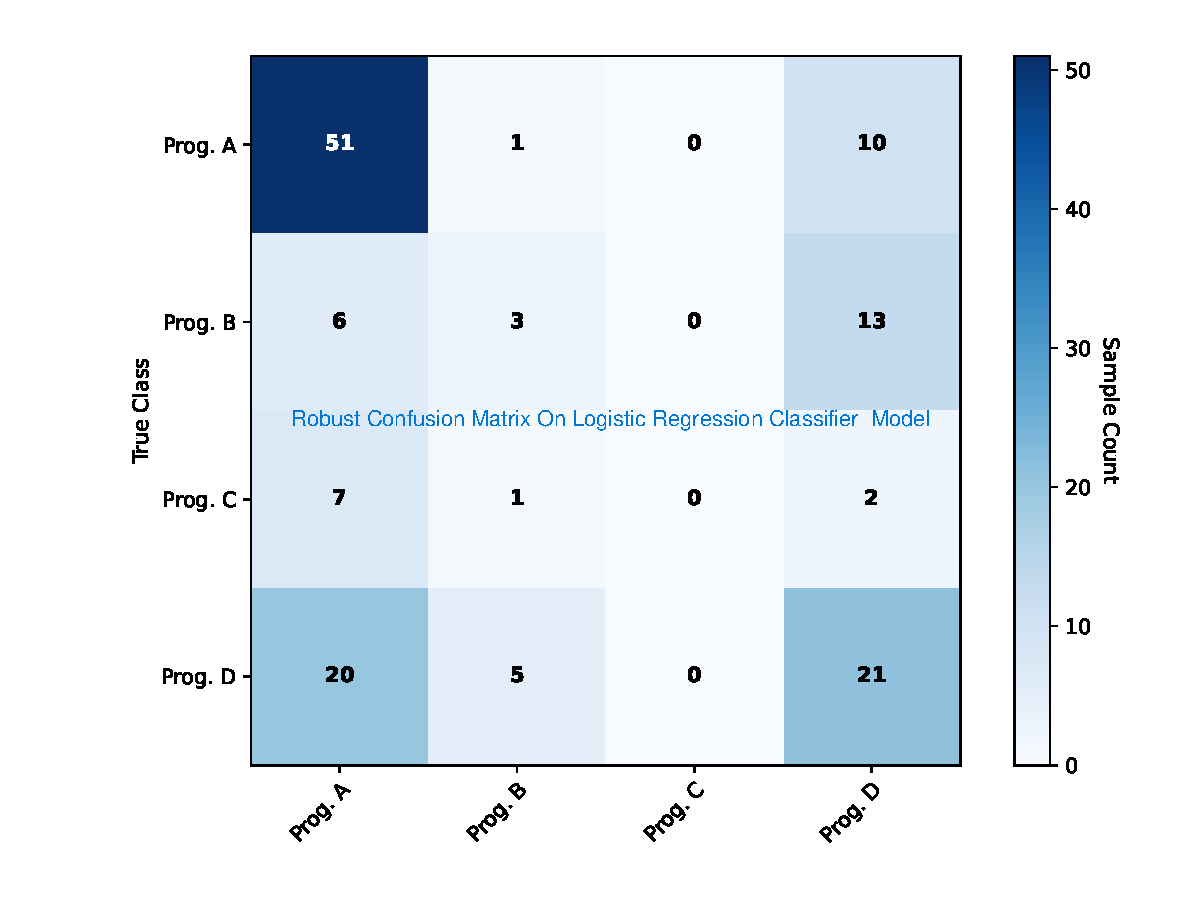
\includegraphics[width=\linewidth]{fig/ROBUST_ConfusionMatrix_1.pdf}
    \caption{Robust}
  \end{minipage}\\
  \begin{minipage}{0.22\textwidth}
    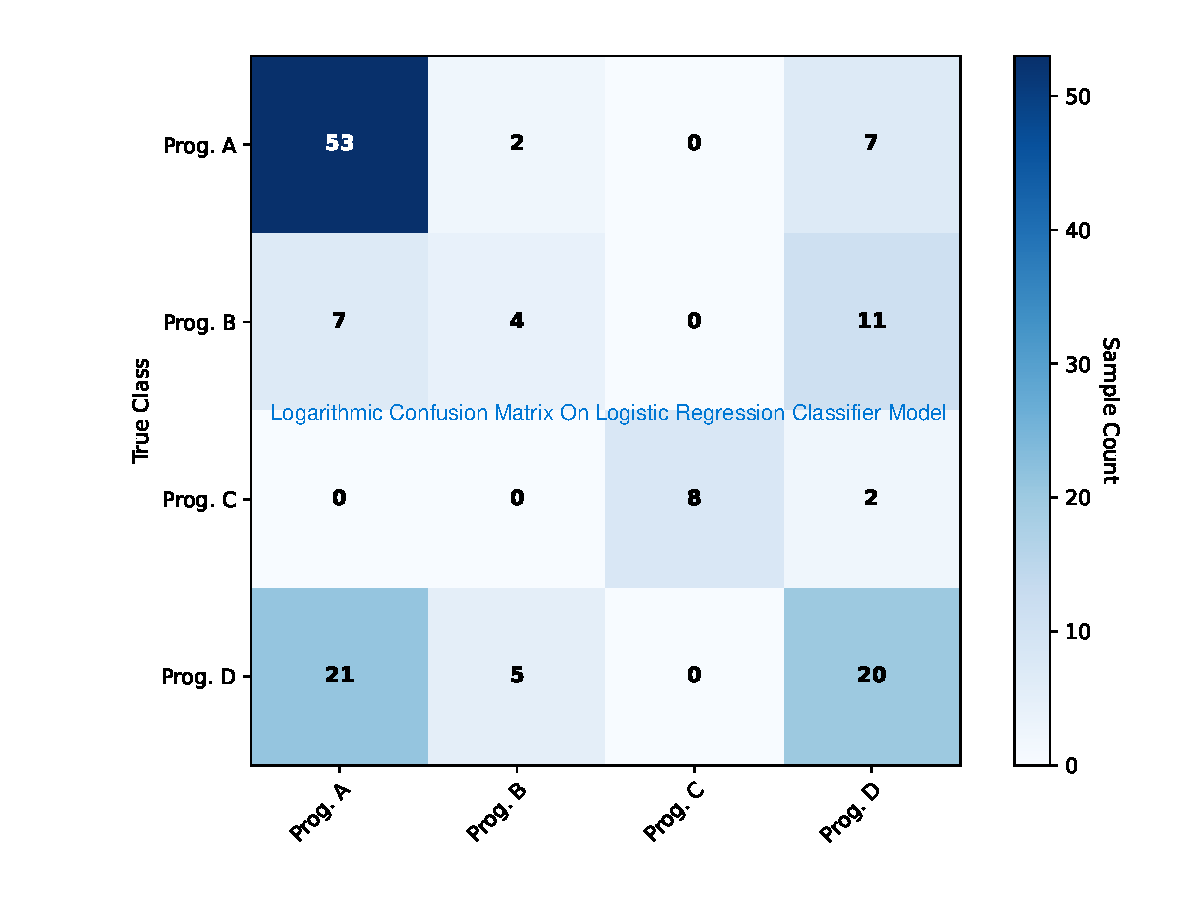
\includegraphics[width=\linewidth]{fig/LOG_ConfusionMatrix_1.pdf}
    \caption{Logarithmic}
  \end{minipage}%
  \begin{minipage}{0.22\textwidth}
    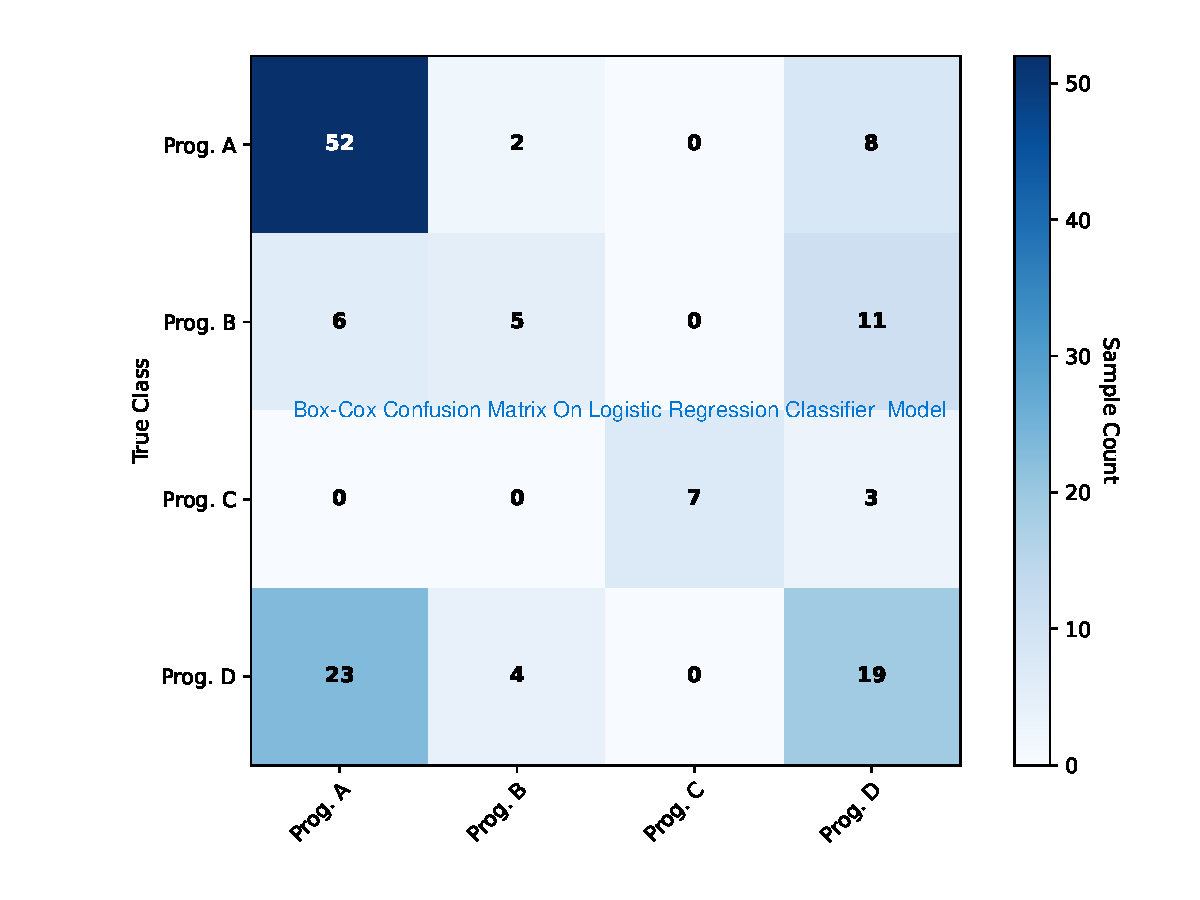
\includegraphics[width=\linewidth]{fig/BOX_COX_ConfusionMatrix_1.pdf}
    \caption{Box-Cox}
  \end{minipage}
  \caption{Confusion Matrix of LR Classifier Model}
  \label{fig:2x2ConfusionMatrixLRClassifier}
\end{figure}

% 接下来是 Boosting-based Classifier 模型，其原数据（未经标准化）的表现力更强，这可能是因为Boosting-based模型通常是基于树的模型，而树模型的一个重要特点是不依赖于特征的缩放，因为它们处理的是特征的分割点，而不是数值的绝对值。因此它可以不适用标准化方法。

For Boosting-based classifiers, the raw (unstandardized) data exhibits stronger performance. This may be because Boosting-based models are typically tree-based models, and a key characteristic of tree-based models is that they do not depend on feature scaling. Since they process split points of features rather than the absolute values of numerical values, they do not require standardization methods.
%在混淆矩阵中只有未处理的数据表现最佳，处理后的数据对于 \textit{Programme} A 分类正确的数量均为47，可能可以说明ensemble learning classifiers对于标准化数据不敏感。
In the confusion matrix, only the untreated data performed best. For the processed data, the number of correctly classified instances for \textit{Programme} A was 47 in both cases, which may indicate that ensemble learning classifiers are insensitive to standardized data.
% 参数和混淆矩阵请见 table II.
See \textbf{Fig. \ref{fig:2x2ConfusionMatrixBoostingBasedClassifier}} and \textbf{Table \ref{tab:BoostingPara}}.

\begin{table}[h!]
    \centering
    \caption{Parameters in Boosting-based Model}
    \begin{tabular}{ll}
        \toprule
        \textbf{Parameters} & \textbf{Value} \\
        \midrule
        n\_estimators & 70\\
        max\_depth & 1\\
        learning\_rate & 0.4\\
        \bottomrule
    \end{tabular}
    \label{tab:BoostingPara}
\end{table}

\begin{figure}[h!]
  \centering
  \begin{minipage}{0.22\textwidth}
    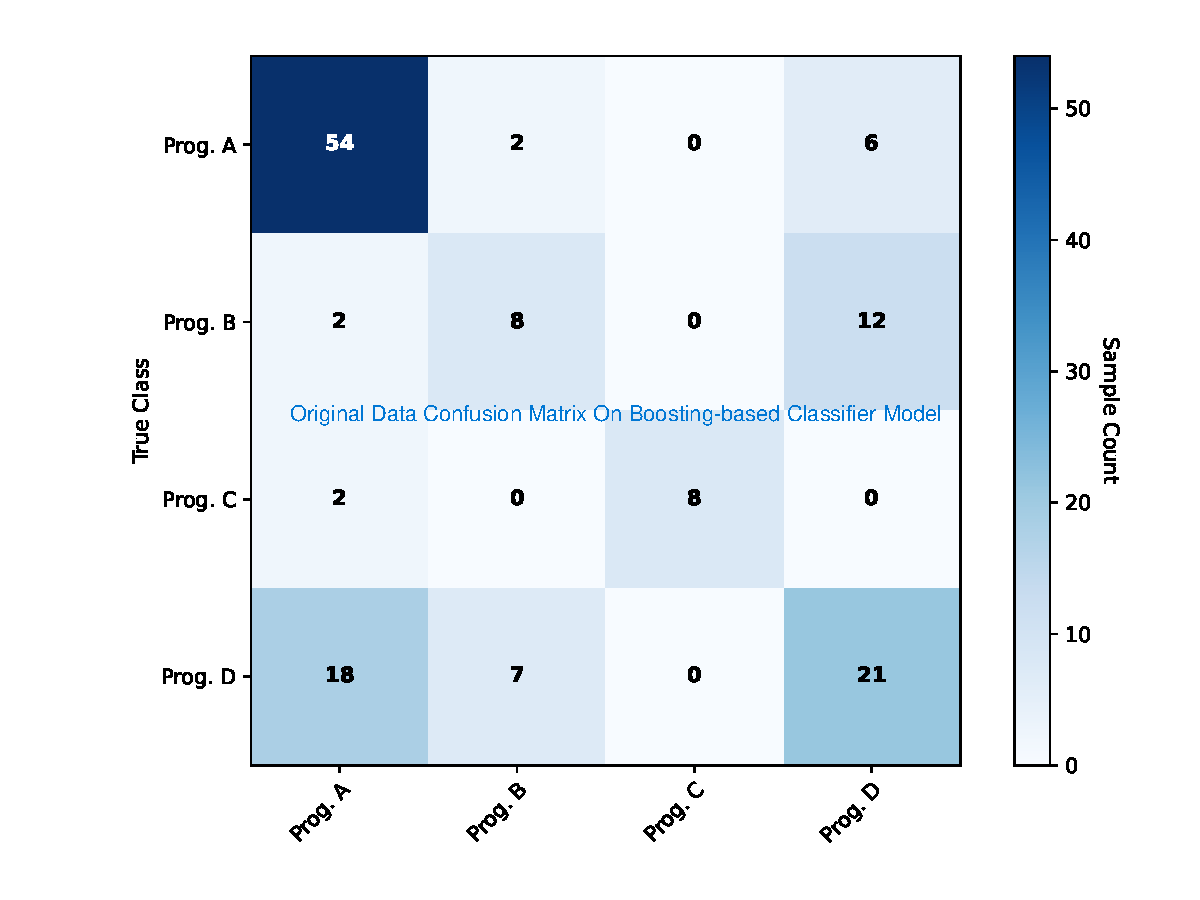
\includegraphics[width=\linewidth]{fig/RAW_ConfusionMatrix_2.pdf}
    \caption{Original}
  \end{minipage}%
  \begin{minipage}{0.22\textwidth}
    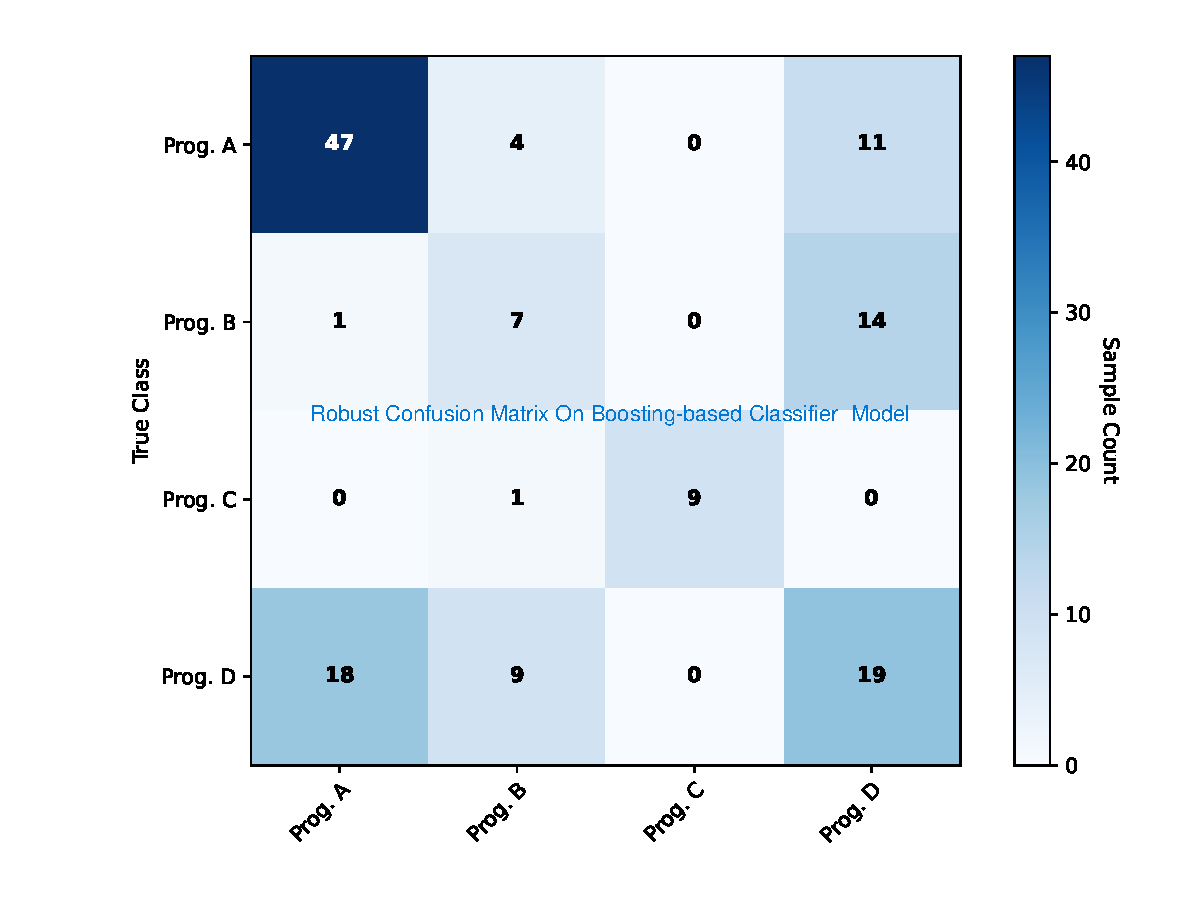
\includegraphics[width=\linewidth]{fig/ROBUST_ConfusionMatrix_2.pdf}
    \caption{Robust}
  \end{minipage}\\
  \begin{minipage}{0.22\textwidth}
    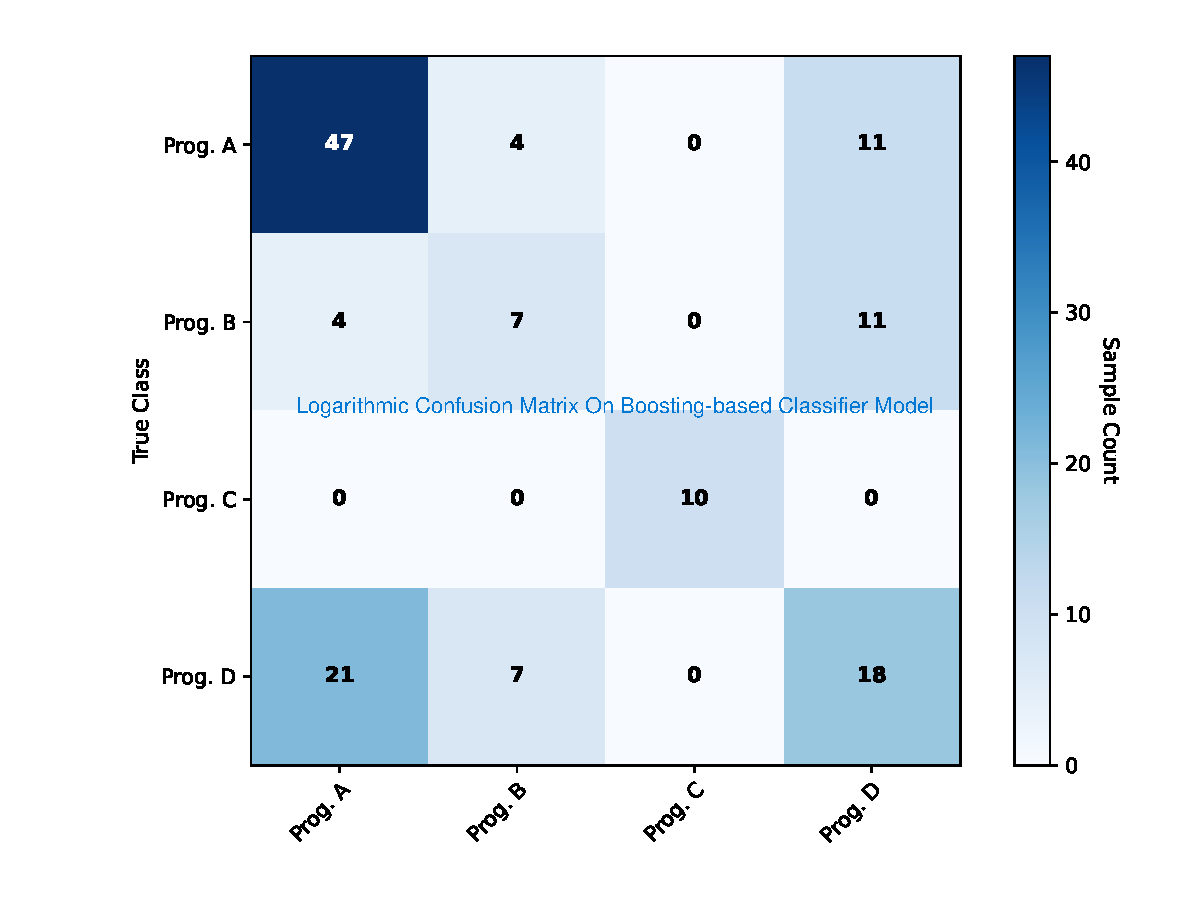
\includegraphics[width=\linewidth]{fig/LOG_ConfusionMatrix_2.pdf}
    \caption{Logarithmic}
  \end{minipage}%
  \begin{minipage}{0.22\textwidth}
    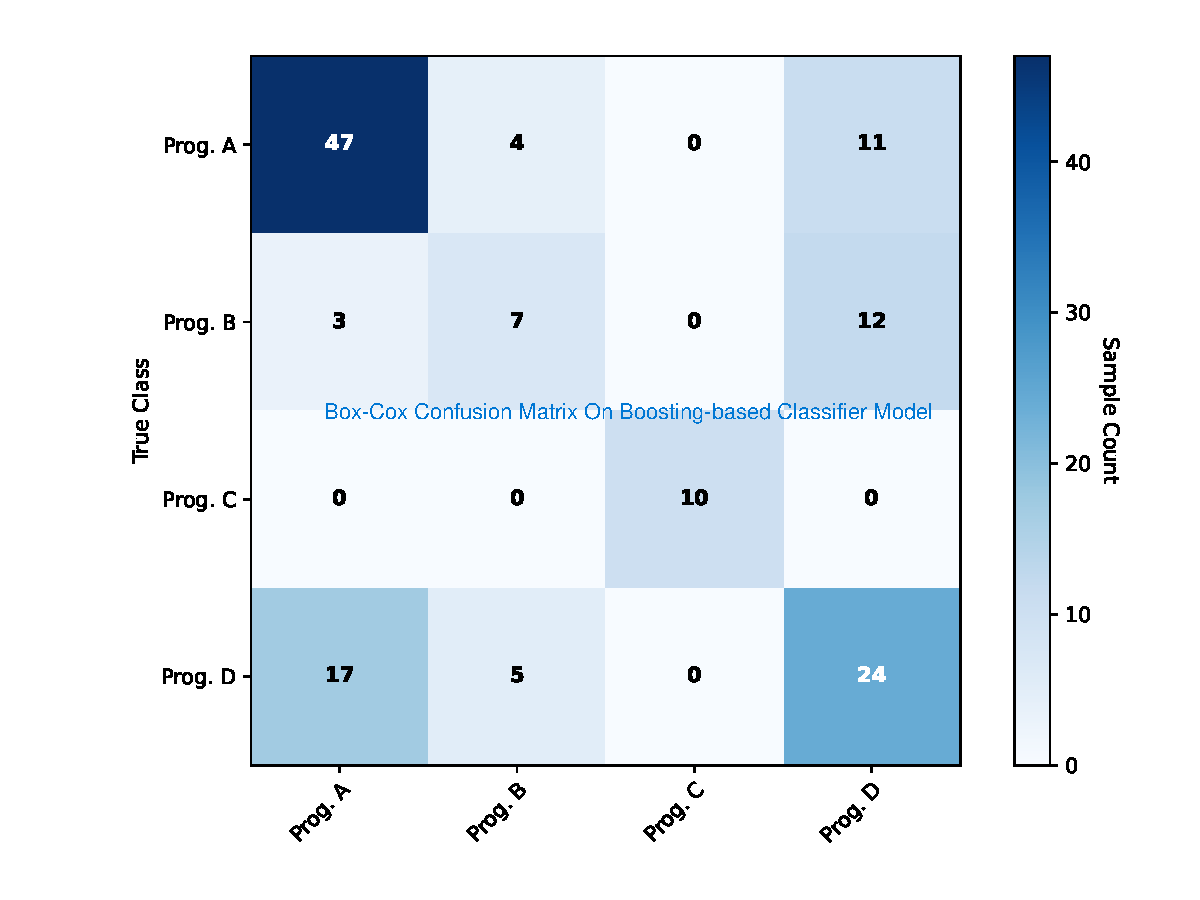
\includegraphics[width=\linewidth]{fig/BOX_COX_ConfusionMatrix_2.pdf}
    \caption{Box-Cox}
  \end{minipage}
  \caption{Confusion Matrix of Boosting-based Classifier Model}
  \label{fig:2x2ConfusionMatrixBoostingBasedClassifier}
\end{figure}

% 最后是Transformer Classification模型，在这个模型中 Box-Cox Standardization的数据表现力十分强力。这在一定程度上和 Boosting-based 模型相反，也就是深度学习分类器对于标准化后的数据表现力强于未标准化后的数据。在训练的过程中设置了输入层11和输出层4，其中中间层（经过不断调试）最优结果是128层。对于训练批次而言设置为32是合理的，如果太低（比如8或者4）则会导致过拟合以及训练结果较慢，而设置为64则会欠拟合，大小为32则是介于两者之间并且有较强的数据泛化能力。而学习率经过不断调整最终找到$1e-3$的大小最佳，Epoch设置为150轮左右其损失函数值稳定在0.69左右。

Finally, in the Transformer classification model, data processed by Box-Cox Standardization exhibits exceptionally strong performance. To some extent, this is the opposite of Boosting-based models—i.e., deep learning classifiers perform better on standardized data than on non-standardized data. During training, the model was configured with an input layer of 11 units and an output layer of 4 units, where the optimal configuration for the hidden layers (after extensive tuning) was 128 units. For the batch size, 32 was deemed reasonable: too small a batch size (e.g., 8 or 4) would lead to overfitting and slower training, while a batch size of 64 would result in underfitting. A batch size of 32 strikes a balance between these extremes and exhibits strong data generalization capability. After repeated adjustments, the optimal learning rate was determined to be $1e-3$. With 150 epochs, the loss function stabilized around 0.69. 
%值得注意的是，虽然在Transformer模型中原始数据表现力比Robust的表现力要好，但是从图中可以明显看出其对\textit{Programme} B 的敏感度（识别率）不如其余三者。因此还需要综合考虑更多因素。
It is worth noting that although the performance of the original data in the Transformer model is better than that of Robust, it can be clearly seen from the figure that its sensitivity (recognition rate) to \textit{Programme} B is lower than the other three. Therefore, more factors need to be comprehensively considered. 
%其混淆矩阵和模型参数请见Fig2
For the confusion matrix and model parameters, refer to \textbf{Fig. \ref{fig:2x2ConfusionMatrixTransClassifier}} and \textbf{Table\ref{tab:TransPara}}
\begin{table}[h!]
    \centering
    \caption{Parameters in Transformer Model}
    \begin{tabular}{ll}
        \toprule
        \textbf{Parameters} & \textbf{Value} \\
        \midrule
        Input Dimension & 11\\
        Output Dimension & 4\\
        Hidden Layer & 128\\
        NHead &2\\
        Num Layer & 3\\
        Epoch & 150 \\
        Learning Rate & 1e-3\\
        \bottomrule
    \end{tabular}
    \label{tab:TransPara}
\end{table}

\begin{figure}[h!]
  \centering
  \begin{minipage}{0.22\textwidth}
    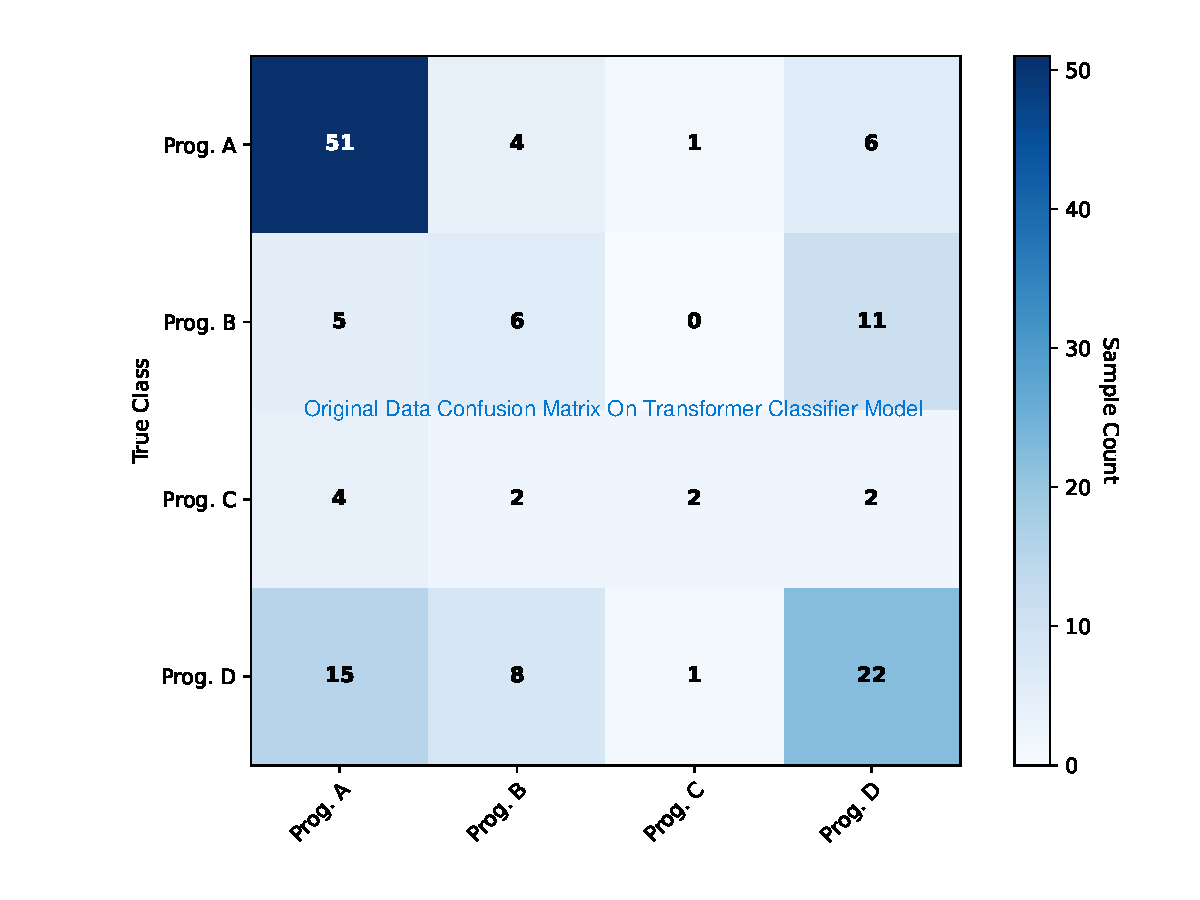
\includegraphics[width=\linewidth]{fig/RAW_ConfusionMatrix_3.pdf}
    \caption{Original}
  \end{minipage}%
  \begin{minipage}{0.22\textwidth}
    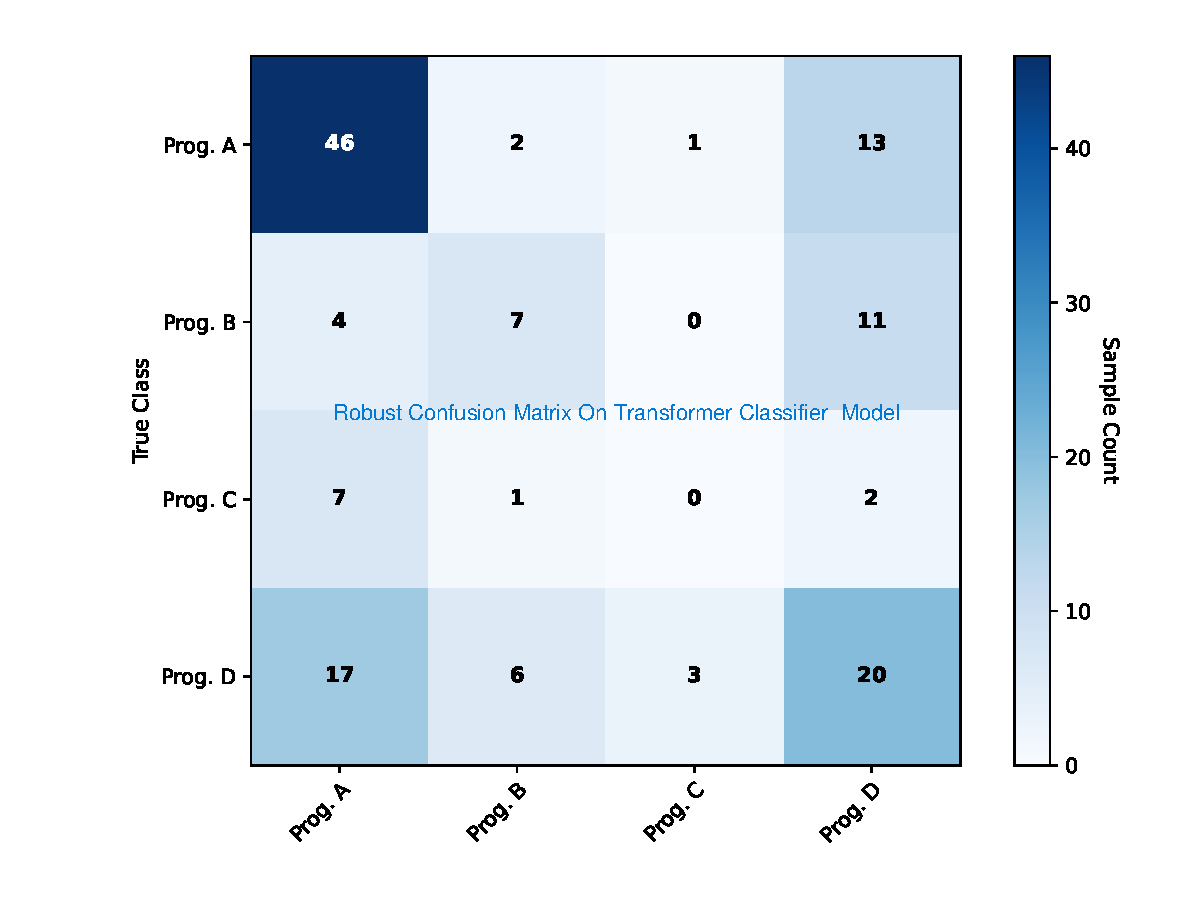
\includegraphics[width=\linewidth]{fig/ROBUST_ConfusionMatrix_3.pdf}
    \caption{Robust}
  \end{minipage}\\
  \begin{minipage}{0.22\textwidth}
    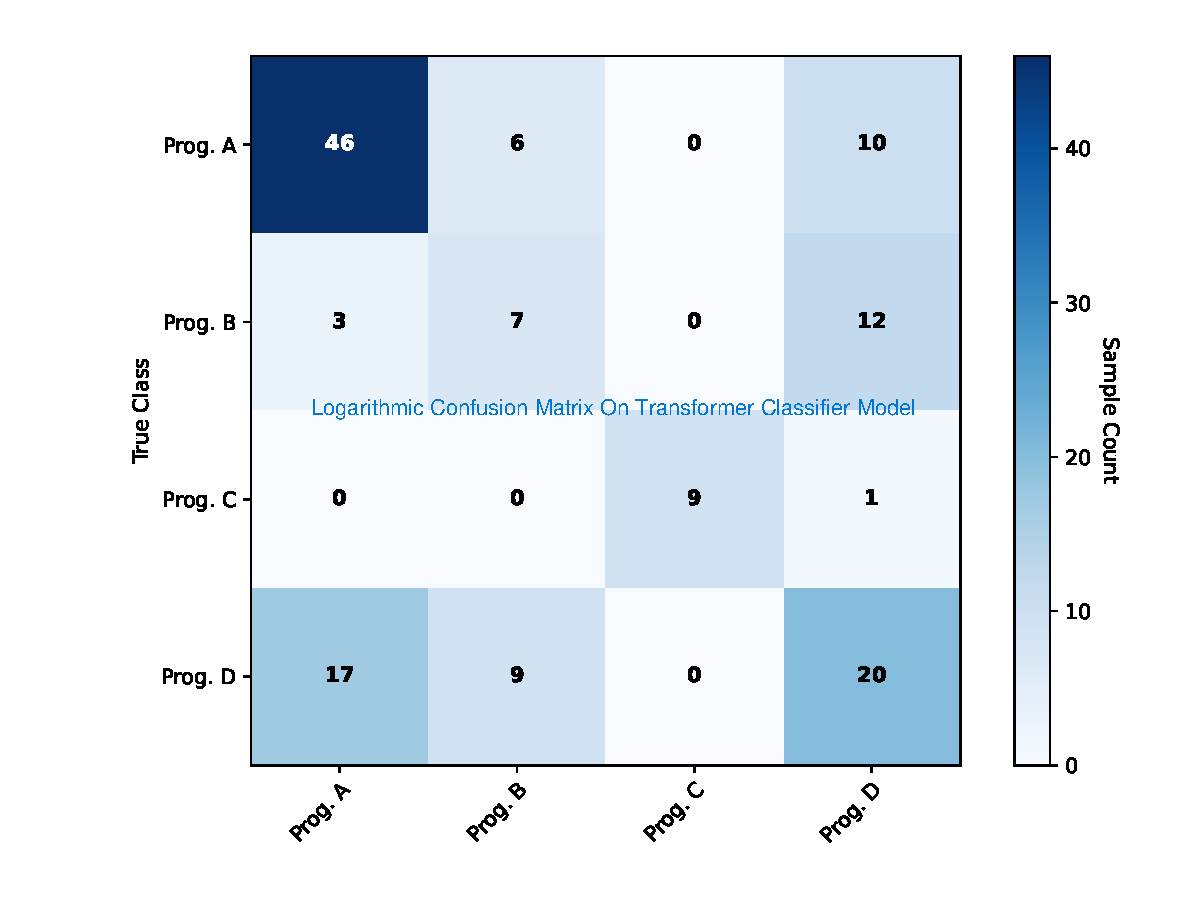
\includegraphics[width=\linewidth]{fig/LOG_ConfusionMatrix_3.pdf}
    \caption{Logarithmic}
  \end{minipage}%
  \begin{minipage}{0.22\textwidth}
    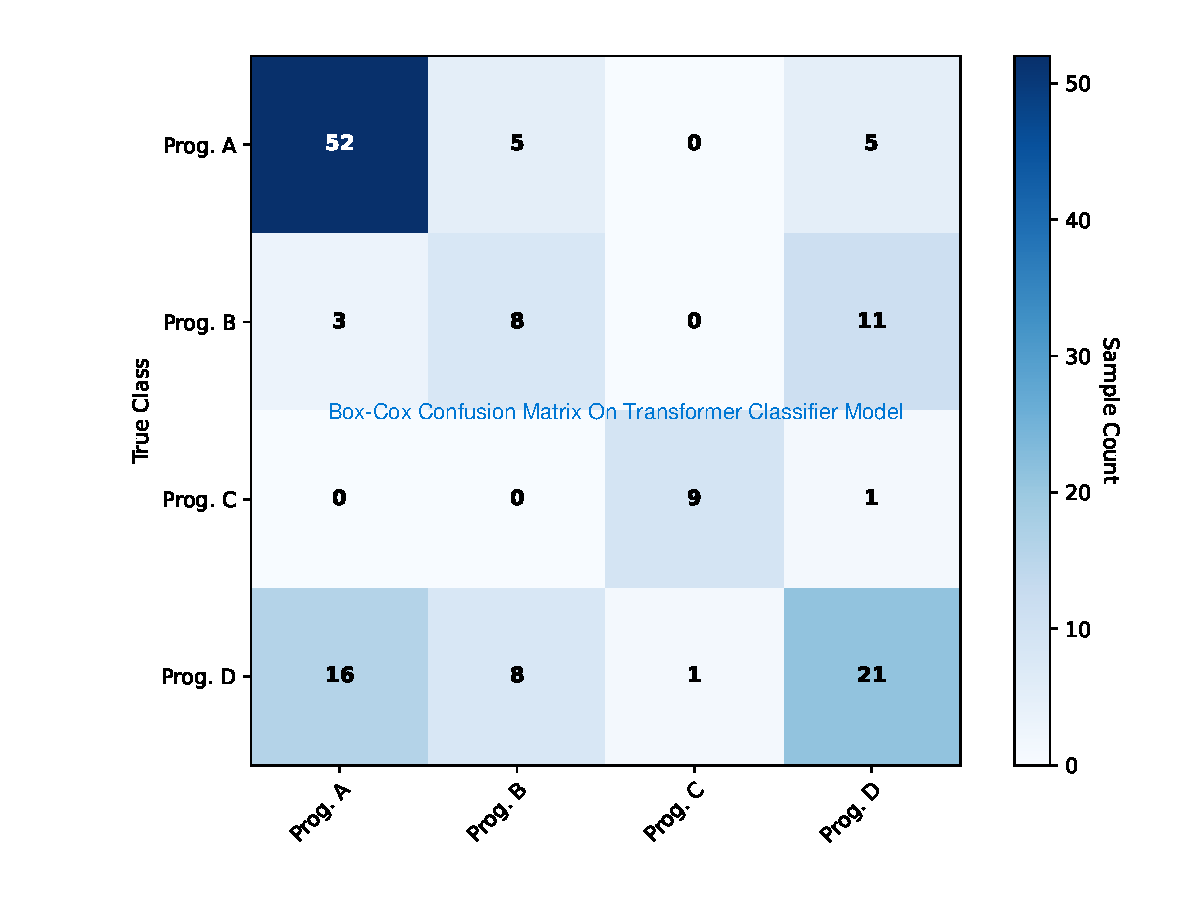
\includegraphics[width=\linewidth]{fig/BOX_COX_ConfusionMatrix_3.pdf}
    \caption{Box-Cox}
  \end{minipage}
  \caption{Confusion Matrix of Transformer Classifier Model}
  \label{fig:2x2ConfusionMatrixTransClassifier}
\end{figure}


\section{\textbf{Conclusion}}
There are some new discovery based on the unsupervised \& supervised learning that mentioned before. In clustering,
% 一旦特征 \textit{Gender} 被加入到了任意一个特征组合之中，经过多次尝试，其聚类效果(基于ARI指标)均不如未加入该特征时的效果。这可以使用 \textbf{Fig. \ref{fig:spearman}} 来说明：因为 \textit{Gender} 该特征与 \textit{Programme} 特征是负相关的。但是对DBI这一指标却无影响，原因是因为DBI是不带标签的聚类评估，而ARI是带标签的聚类评估。DBI的簇间距离和簇内距离的比值不会受到负相关的影响。
once the feature \textit{Gender} is added to any feature combination, after many attempts, its clustering effect (based on the ARI index) is worse than that without adding this feature. This can be illustrated by \textbf{Fig. \ref{fig:spearman}}: because the feature \textit{Gender} is negatively correlated with the feature \textit{Programme}. But it has no effect on the DBI index. The reason is that DBI is a label - free clustering evaluation, while ARI is a label - based clustering evaluation. The ratio of inter - cluster distance to intra - cluster distance in DBI will not be affected by negative correlation. 

% 第二，在分类（监督学习）中发现，传统机器学习（逻辑回归分类模型）对数据标准化敏感，对于那些标准化后的数据往往能得到更好的准确度。而对于Ensemble learning classifiers则不敏感，因为原始数据比 Robust和 Logarithmic 标准化的准确率要高得多，但是仅仅略高于 Box-Cox 标准化。此外，对于Transformer模型，只有经过 Box-Cox 标准化后的数据表现出色，其余标准化或者没有标准化的数据表现不佳，因此得出结论：它和传统机器学习一样对数据标准化敏感

Secondly, it is found in classification (supervised learning) that traditional machine learning (logistic regression classification model) is sensitive to data standardization and often achieves better accuracy for those standardized data(see \textbf{Fig. \ref{fig:accuracyResult}.}). However, for Ensemble learning classifiers, they are not sensitive, because the accuracy of the original data is much higher than that of Robust and Logarithmic standardization, but only slightly higher than Box - Cox standardization. Furthermore, for the Transformer model, only the data standardized by Box - Cox perform well, while the data with other standardizations or no standardization perform poorly. Thus it is concluded that it is as sensitive to data standardization as traditional machine learning.  

% 此外，在聚类和分类这两个任务中，通常发现 Robust 标准化远不如 Logarithimic 和 Box-cox 标准化，一个可能的想法是，数据有偏态（这一点在Section II 已说明）的情况下，比如学生某些\textit{Question} 成绩高分多，对数变换能调整分布，让数据更均匀，标准化后各特征权重更合理。而 Robust 标准化虽然抗噪，但可能把数据压缩太厉害，丢失一些区分信息。但是正是这些特别的信息能够让模型更好的识别出这个学生属于哪个专业。比如 K-means 这类聚类对数据分布有假设，正态化后效果更好。分类模型如逻辑回归，标准化后梯度下降更快，而对数处理后的数据可能让特征间关系更线性，提升模型表现。

Furthermore, in both clustering and classification tasks, Robust standardization is generally found to be far less effective than Logarithmic and Box-Cox standardization. A possible explanation is that when the data is skewed (as discussed in Section II)—for example, students have many high scores on certain \textit{Q} items—logarithmic transformation adjusts the distribution to make the data more uniform. After standardization, this ensures more reasonable feature weights. Although Robust standardization is noise-resistant, it may over-compress the data and lose some discriminative information. However, it is precisely this unique information that allows the model to better identify which major a student belongs to. For instance, clustering algorithms like K-means make assumptions about data distribution, and performance improves when data is made more normally distributed. In classification models such as logistic regression, standardization accelerates gradient descent, while logarithmically transformed data may linearize relationships between features, enhancing model performance.

% 最后，对于未来的工作，在分类中可以考虑加入更多的模型例如随机森林等并且使用集成学习来提升准确率。在聚类方面可以考虑收集更多的学生信息数据来提升ARI和DBI聚类效果。
Finally, for future research, in the classification task, we can consider incorporating more models such as Random Forest and utilizing ensemble learning to enhance accuracy. In the clustering task, collecting more student profile data can be explored to improve the clustering performance measured by the ARI and DBI.






































\bibliographystyle{ieeetr}
\bibliography{reference}
\end{document}
